\documentclass[a4paper]{report}
\usepackage{setspace}
%\usepackage{subfigure}

\pagestyle{plain}
\usepackage{amssymb,graphicx,color}
\usepackage{amsfonts}
\usepackage{latexsym}
\usepackage{amsmath}
\usepackage[a4paper, margin = 3cm, bottom = 2.5cm]{geometry}
\usepackage{tabularx}
\usepackage{xltabular}
\usepackage{booktabs}
\usepackage{float}
\usepackage{longtable}
\usepackage{tikz}
\usepackage{hyperref}
\usepackage{listings}
\usepackage{pgfplots}
\usepackage{multicol}
\usepackage[backend=biber, style=numeric-comp, sorting=none, url=true]{biblatex}
\addbibresource{main.bib}

\usetikzlibrary{arrows.meta, bending}


\lstset{basicstyle=\ttfamily\small}
\newtheorem{theorem}{THEOREM}
\newtheorem{lemma}[theorem]{LEMMA}
\newtheorem{corollary}[theorem]{COROLLARY}
\newtheorem{proposition}[theorem]{PROPOSITION}
\newtheorem{remark}[theorem]{REMARK}
\newtheorem{definition}[theorem]{DEFINITION}
\newtheorem{fact}[theorem]{FACT}

\newtheorem{problem}[theorem]{PROBLEM}
\newtheorem{exercise}[theorem]{EXERCISE}
\def \set#1{\{#1\} }

\newenvironment{proof}{
PROOF:
\begin{quotation}}{
$\Box$ \end{quotation}}



\newcommand{\nats}{\mbox{\( \mathbb N \)}}
\newcommand{\rat}{\mbox{\(\mathbb Q\)}}
\newcommand{\rats}{\mbox{\(\mathbb Q\)}}
\newcommand{\reals}{\mbox{\(\mathbb R\)}}
\newcommand{\ints}{\mbox{\(\mathbb Z\)}}

%%%%%%%%%%%%%%%%%%%%%%%%%%


\title{{\vspace{-14em} 
\includegraphics[scale=0.4]{ucl_logo.png}}\\
{\Huge Clinical Summarisation and Advice for Intel AIPC}\\
}
\date{Submission date: 1st May 2026}
\author{22004608\thanks{
{\bf Disclaimer:}
This report is submitted as part requirement for the Meng Computer Science degree at UCL. It is
substantially the result of my own work except where explicitly indicated in the text.
\emph{Either:} The report may be freely copied and distributed provided the source is explicitly acknowledged
\newline  %% \\ messes it up
\emph{Or:}\newline
The report will be distributed to the internal and external examiners, but thereafter may not be copied or distributed except with permission from the author.}
\\ \\
Meng Computer Science\\ \\
Prof. Dean Mohamedally (UCL), Costas Stylianou (Intel)}



\begin{document}
 
\onehalfspacing
\maketitle

\pagenumbering{roman}
\begin{abstract}
GPs spent on average 25\% of their working day handling clinical paperwork and updating Electronic Patient Records (EPR) systems. This application aims to ease the stress and time taken by medical professionals by harnessing an Ambient Voice Technology (AVT) approach to record, transcribe, diarise, and summarise medical consultations to reduce time spent during and after consultations taking notes and follow-up reports. Furthermore, the appraisals feature allows doctors to generate appraisal entries by supplementing the summarisation with additional appraisal notes and tags. These entries can be viewed in the history and searched for by name or tag. Finally, by enabling the doctor to upload medical guidance documentation, the application will search for relevant guidelines to enable the GP to explore and cite medical advice based on the conversation. By engineering this project as an offline application, we expand the use case to in-home visits and ensure that all sensitive data is safe due to not requiring an internet connection for any part of the application. This application aims to reduce the time taken recording notes and inputting data into EPR systems by providing concrete transcripts, summarisations and medical advice based on the consultation.

An iterative approach allowed for flexibility in the project's development, allowing for the feedback from supervisors and healthcare professionals to be quickly integrated into the current solution. This project built on a summer project using an Intel Gaudi server running a LLM to summarise patient-doctor consultations. This was extended further to move the application onto the Windows platform, running entirely offline with the additional transcription pipeline and a RAG model for the search for relevant medical guidelines.

This project harnesses the power of Intel's AIPCs by using OpenVINO to quantise machine learning models to reduce the inference time resulting in an increase in speed and decrease in application size, producing fast and accurate summarisations of medical conversations, with medical advice provided if required.
\end{abstract}

\chapter*{Acknowledgements}
I would like to take this time to acknowledge the people around me who made this possible. Thank you to both Costas and Dean for their timely and unwavering support throughout this project. Their understanding of my personal deadlines this year and passion for promoting this project combined with their expertise around marketing and implementation resulted in a smooth and effective development process. 
I would like to further thank my friends and flatmates. Without the knowledge and support from Jasper, James and the rest of "Hello World" I would not be in the position I'm in today. 
Finally, my family and loved ones have created an incredible support system around me, picking me up through the challenges, and celebrating my successes, through my UCL journey.


\tableofcontents
\clearpage
\pagenumbering{arabic}

\chapter{Introduction}
This research investigates the application of on-device machine learning to summarise clinical consultations. As a proof-of-concept, the primary objective is to evaluate the feasibility of an offline machine learning pipeline running on Intel AI PC hardware. This aims to reduce an NHS GP's workload by autonomously recording and transcribing consultations, generating clinical summaries, and retrieving medical guidance within an entirely offline environment. 

While existing cloud-based systems such as TORTUS AI, Heidi Health, and Nuance DAX Copilot highlight the utility of automated clinical documentation within healthcare, they rely on networked deployment, extensive integration, and external data processing \cite{tortus_product_2026,heidi_product_2026,dictationdirect_dax_features_2026}. In the context of the NHS, these dependencies introduce significant data governance and infrastructural challenges. Consequently, developing an offline proof-of-concept provides a mechanism to evaluate an alternative deployment architecture designed to address these specific operational constraints.

This project was developed as part of the UCL IXN in partnership with Intel with consultation from Dr. Atia Rafiq, an NHS GP and GP trainer and Dr. Tazeen Ahmed an NHS Rheumatology Care Group Lead.

\section{Problem Overview}
In a consultation, a doctor needs to listen, ask follow-up questions, reason about symptoms, and still produce a record that is accurate for later clinical use. The usual consultation flow is as follows: type and take notes during the appointment, ask follow-up questions, and reconstruct the encounter afterwards. Each of these stages has their drawbacks. Typing during the consultation interrupts eye contact and changes the rhythm of the conversation and writing notes afterwards is slow and risks losing detail.

The main idea of this project is to shift the administrative work into an on-device pipeline. The application records the conversation, transcribes and diarises (labelling sentences as doctor or patient) in real time, produces a clinical summary after the consultation, and searches uploaded guidance documents for relevant medical guidelines. In practice, the output of the consultation contains a transcript, a summary, and a link back to guidance that may help the clinician check what was discussed. This provides a practical basis for evaluating whether an offline workflow can support useful clinical documentation without relying on cloud services.

Running the full pipeline locally introduces its own problems. Large language models are expensive to run. All models must be fast to load and infer enabled by an adequately designed concurrent pipeline ensuring the application remains responsive. Retrieval and summarisation has to be fast, otherwise it becomes one more waiting step in an already busy workflow. The system also has to fit into the constraints of the target platform, a native Windows Store application built with the MSIX packaged project platform and deployed as an MSIX package on Intel AI PC hardware.

\section{Aims}
The project has three main aims:

\begin{itemize}
    \item Evaluate whether the selected models and libraries are fast enough and accurate enough to support an offline workflow in practice.
    \item Build a working proof of concept for offline clinical summarisation on Intel AIPC hardware, with a native Windows user interface and an entirely local inference pipeline.
    \item Produce a codebase and architecture that can be extended after the project, rather than a one-off demonstration that is difficult to maintain.
\end{itemize}

A personal secondary aim is established based on the project requirements. The majority of my development experience throughout my university journey is with Python and VSCode. The technical constraints of this project provide the opportunity to learn the C++ programming language, the Visual Studio environment and the MSIX Packaged Project platform. 

\section{Goals}
From those aims, I defined the following concrete project goals:

\begin{itemize}
    \item Compare candidate pre-trained medical large language models (LLMs) under different quantisation levels and select a summarisation model that is feasible on the target hardware.
    \item Build an Ambient Voice Technology (AVT) pipeline to record and transcribe conversations
    \item Build a retrieval pipeline that allows clinicians to upload medical guidance PDFs and locate relevant sections from the generated consultation summary.
    \item Provide a Windows-native interface for recording, reviewing outputs, selecting and saving external files, and browsing retrieved guidance.
    \item Structure the application so that future work, such as appraisal support or EPR integration, can be added without major rewrites.
\end{itemize}

These goals are intentionally narrower than the long-term ambitions of the product idea. For example, direct EPR integration, multilingual support, and patient-facing summaries are useful extensions, but they are not required to establish whether the core offline pipeline is viable for this proof-of-concept project.

\section{Development Methodology}
This project was set out with two phases, feasibility followed by iterative development on a 1 week cycle. Initially a feasibility study was conducted to determine whether latency and accuracy within the summarisation pipeline could remain within the requirement specification. This involved testing candidate models by measuring inference times, and evaluating performance on a summarisation benchmark.

Development began once technical this feasibility study concluded. Weekly meetings with my external supervisor and regular discussion with my internal supervisor and the NHS clients expanded the small starting feature pool. The original requirements were deliberately narrow, focusing only on local summarisation. Through demonstrations and feedback collection, the scope broadened to include AVT, medical guidance retrieval, and appraisal entries. 

The project is maintained on GitHub, which makes it practical to isolate experiments, preserve stable versions for demonstrations, and revert changes when a promising approach had flaws that required a reset to fix. This mattered most when integrating several highly linked libraries simultaneously with very different potential points of failure.

This flexible development lifecycle suited a proof-of-concept project with several unknowns and regularly evolving requirements. By prioritising high-risk ambiguities in the requirements at the start of development, a stable baseline could be set for demonstrations, thus pre-empting repository refactors due to sudden shifts in requirements.

\section{Overview}
The remainder of this report is organised as follows.

Chapter 2 reviews the background to the project, surveys comparable systems, and explains the choice of models, frameworks, and supporting libraries.

Chapter 3 defines the project requirements in detail and analyses the consequences of those requirements for the system architecture, data model, workflows, and stakeholder responsibilities.

Chapter 4 describes the design and implementation of the application, including the structure of the main components and the reasoning behind the architectural decisions.

Chapter 5 presents the testing strategy, summarises the evidence gathered during development, and identifies the main limitations of the current proof of concept.

Chapter 6 reviews the project against its original goals, critically evaluates the resulting system, and outlines the most important directions for future work.
\chapter{Context and Background Information}
% This chapter should cover background information, related work, research
% done, and tools or software selected for use in the project.
% – Provide necessary context and background information to describe
% how your project relates to what is already known or available.
% – A description of the research carried out to learn out about the nature
% of the problem(s) being investigated and potential solutions. The form
% of the research will vary widely depending on the kind of project. For
% example, it might involve searching through research publications and
% online resources, or might involve an exploration of design
% possibilities for a user interface or program structure.
% – The sources of information you are drawing on (papers, books,
% websites, etc.) should all be cited or referenced clearly. In addition,
% state how each source relates to your work and avoid the temptation
% to pad out the chapter by including sources that you didn’t make use
% of during the project.
% – If relevant, a survey of similar solutions, programs or applications to
% yours, and how yours is differentiated.
% – Introduce the software, programming languages, library code,
% frameworks and other tools that you are using. Discuss choices and
% make clear which you made use of and why.
% You should not include well known things (e.g., HTML or Java) or try to give
% tutorials on how to use a tool or code library (use references to books and
% websites for that information). Everything you include should be directly
% relevant to your work and the relationship made clear. This chapter is likely
% to be fairly substantial, perhaps 8-10 pages.

% You should provide enough background to the reader for them to understand what the project is all about. For example:
% • What problem are you solving?
% • Why are you solving it?
% • How does this relate to other work in this area?
% • What work does it build on?
% • What is the scope of your work?
% • What is included in the scope and what is outside the scope?

\section{Background Information}
\subsection{OpenVINO}
The Intel Open Visual Inference and Neural Network Optimization (OpenVINO) toolkit is an open-source software stack designed to facilitate the rapid optimisation and deployment of machine learning models on Intel AIPC hardware\cite{intel_openvino_genai_workflow_2026}. Although the original release in May 2018 focused on computer vision tasks, it has received yearly updates following industry movement towards LLMs and generative AI\cite{intel_openvino_launch_2018}. One large benefit of this toolkit is the `optimum-cli` tool, enabling the download, quantisation, and conversion to OpenVINO intermediate representation (OpenVINO IR)\cite{intel_openvino_gaudi_aipc_2024}. The tool converts any huggingface model to OpenVINO IR format. If quantisation is required, it uses the Neural Network Compression Framework to reduce the mathematical precision of the model's weights, reducing the storage size and inference time with a negligible trade-off of inference accuracy\cite{hybrid_llm_openvino_2024}. It then exports the model into a .xml file mapping the network configuration and a .bin file containing the model's weights to satisfy the OpenVINO IR format. The OpenVINO inference engine executes the OpenVINO IR model using an optimised C++ engine directly interacting with low level hardware instruction sets on Intel's AIPC system-on-a-chip (SOC) architecture\cite{intel_openvino_inference_engine_2023}.

\subsection{Intel AI PC}
The Intel AIPC series was launched in December 2023 transitioning away from the old architectures of separately dedicated CPU, GPU and RAM components and moving towards a SOC design\cite{intel_meteor_lake_2023} where the previous components and new Neural Processing Unit (NPU) all live on the same combined chip stack by the release of the Lunar Lake series in late 2024. The NPU was a new computational unit specialised for low power matrix computation, designed as a device for low power inference of small ML models\cite{intel_lunar_lake_2024}. When paired with the native OpenVINO inference engine, the Intel AIPC is a strong candidate to provide a proof-of-concept for locally hosted ML pipelines\cite{fei2024_nitro_openvino}.

\subsection{Ambient Voice Technology}
Ambient Voice Technology (AVT) is an umbrella term for the field of passive automated note taking during conversations. The standard pipeline is as follows:

\begin{figure}
    \centering
    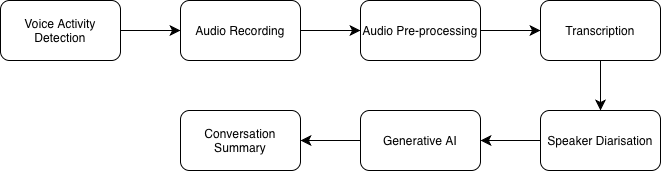
\includegraphics[width=1\linewidth]{AVT_diagram.drawio.png}
    \caption{A typical AVT workflow}
    \label{fig:AVT_diagram}
\end{figure}

This pipeline takes an audio stream as input, providing a summary as output \cite{lakhani_ai_scribes_2025}. Within the medical section this pipeline has been implemented with specialised speech-to-text and summarisation models to produce standardised medical documentation from a medical conversation \cite{tortus_product_2026}

\subsection{RAG}
Retrieval Augmented Generation (RAG) is a technique that enhances generative model outputs by first retrieving contextually relevant information from an external knowledge base and conditioning the model's generation on that retrieved context\cite{lewis_rag_2020}. This addresses a fundamental limitation of parametric LLMs. Since knowledge is fixed at training time, reliable access to domain specific or recently updated information is impossible without model retraining. The retrieval stage converts both the query and the knowledge base documents into dense vector representations (embeddings) using a semantic encoder. These embeddings capture the contextual meaning of text, enabling semantically similar passages to be located without exact keyword overlap. An approximate nearest neighbor (ANN) algorithm then searches the embedding index to surface the most contextually relevant document chunks\cite{malkov_hnsw_2020}. The retrieved chunks are passed to the LLM as additional context, enabling grounded responses anchored in verified source documents and significantly reducing the hallucination of domain-specific facts\cite{gao2023retrieval}. 

\subsection{NHS Appraisals}
Medical appraisals are an annual meetings with a supervisor aimed at retrospectively assessing challenges and lessons learnt from a personal development plan\cite{nhs_england_what_is_appraisal}. During this process, doctors must review their practice, evaluate patient and colleague feedback, and establish continuous personal development plans \cite{gmc_appraisal_guidance}. A method of reviewing their practice is through ad-hoc notes on specific consultations. An AVT solution can alleviate some of the pressure of gathering supporting information from consultations by storing reflection notes until an appraisal is required. This integration was requested by Dr. Atia Rafiq to aid her trainee GP's through this process

\subsection{Project Ambience (LLMedic)}
The prequel to this project, developed over the summer 2025 at UCL, hosted the Med42-70B model used for medical summarisation on Intel's GAUDI compute servers designed for AI acceleration on Intel hardware\cite{intel_gaudi3_2025}. This project acted as a proof-of-concept for running large AI fine-tuned medical models on Intel hardware using a web application for a client-server distribution model. The main shortfall was the hosting architecture as this server has open access to UCL students on a root level account, resulting in a solution too insecure to handle sensitive data. To remedy this, the project requires moving this model to an offline, on-device solution \cite{intel_openvino_gaudi_aipc_2024} while extending the summarisation pipeline with an AVT approach, appraisal entry system and RAG for medical advice. 

\section{Evaluation of Similar Solutions}
Evaluating the capabilities and shortfalls is essential to building a unique application that can capture the pain points of the current applications available to enable this proof of concept project to target a gap in the market. Furthermore, by analysing the current solutions, this project can position itself to develop on the successes that other applications have achieved in this growing field. 

\subsection{TORTUS AI}
TORTUS AI is an ambient medical scribe developed for the NHS as part of Great Ormond Street Hospital's (GOSH) drive for digital innovation involving a pipeline of machine learning models achieving an AVT and AI-scribe solution with complete integration into the GOSH EMIS EPR system\cite{tortus_product_2026}. This solution creates a "clinician in the loop" to systematically categorise LLM errors into risk levels targeting hallucinations and omissions from summaries during the training of their summarisation model on 13000 clinician annotated statements\cite{tortus_creola_2026}. Rollouts of this solution have shown a 23.5\% increase in face to face interaction between patients and doctors during consultations with an 8.2\% decrease in consultation length\cite{gosh_implementing_ai_2025}. In high pressure environments such as A\&E, the deployment of this solution enabled doctors to treat 13.4\% more patients per shift\cite{nia_tortus_2025}. Overall this is the leading solution for AVT and AI-scribe technologies in the NHS.

Considering the features of this project's solution, TORTUS AI does not support functionality for citing medical guidelines, or an appraisal entry solution. Furthermore, the key differentiating factor is the platform these applications will be hosted on. TORTUS uses a server-client network strategy, requiring a stable internet connection and complex network configuration within each NHS hospital and practice compared to our offline solution.

\subsection{Heidi Health}
Heidi health is a the UK's largest AVT solution founded in Australia. This solution is the UK's largest clinical rollout of AVT with the Modality Partnership, the NHS's largest GP super-partnership serving 360 GPs\cite{heidi_modality_2026}. This solution enables multi-language support along with generating subjective, objective, assessment, plan (SOAP) notes, referral letters, patient explainers and medical code suggestions with UI customisation and a large range of platforms. Due to this solution having a global scale, support for EHR integration is not yet possible\cite{deepcura_heidi_review_2026}. This platform also contains a "Context" feature allowing clinicians to upload patient documents, notes and clinical guidelines to provide the "Ask Heidi" chatbot with patient data\cite{heidi_product_2026}. Evaluating the pilot of this solution with 47 primary care doctors, Heidi state a clinicians experienced a 61\% reduction in after-hours admin and a 51\% reduction in documentation time during appointments resulting in 78\% of clinicians stating they build a better rapport with patients\cite{colcol_ai_adoption_2026}. Heidi have also recently rolled out a hybrid solution allowing Doctors to attach a proprietary clip-on microphone to capture conversations offline then connecting to the online system once convenient to then integrate with the current Heidi system\cite{wells_heidi_hardware_2026}. 

This solution trades off EPR integration for extensive UI customisation compared to TORTUS resulting in the comparison between Heidi and this project being identical to the previous comparison of TORTUS and this project. The extension that heidi provides is a workaround to gain offline capabilities, however requires the purchase and carrying of a proprietary device.

\subsection{Nuance DAX Copilot (Microsoft)}
Nuance Dragon Ambient eXperience (DAX) Copilot is an ambient AI solution by Nuance Communications, acquired by Microsoft. This harnesses the Azure's secure cloud infrastructure designed to scale with EPR integration in zero-trust security environments. In the context of our NHS domain, this solution has native integration with the EPIC EPR system through Dragon Medical One, while harnessing Microsoft's RAG capabilities within the hospital trust's database by ingesting the database based on a configuration for an enterprise-level RAG solution\cite{dictationdirect_dax_features_2026}. Total Voice Technologies, a retailer of DAX, claim that clinicians saved 7 minutes per encounter with 70\% of clinicians reporting a reduction of fatigue during and after consultations while capturing 75\% more information\cite{totalvoicetech_dax_2026}.

This is a very well rounded solution harnessing the power of Microsoft's cloud computing to create a central knowledge bank which can be automatically updated and queried. Again similar to the previous solutions, there is no native capability to handle remote consultations where a stable wifi connection and hospital network access is difficult and not guaranteed.

\subsubsection{Conclusion}
To conclude, although solutions in this field already exist, our unique approach of a completely offline open-source approach with the addition of integrating medical guidelines positions this project in a unique area. This negates the drawbacks of requiring network and server setup or proprietary devices along with the safety of sensitive data transmission over a network. After researching for completely offline on-device solutions, none were found at the time of writing for a clinical application. By attempting to capture the many benefits of these different applications while maintaining an offline solution, this project will act as a proof of concept for locally hosted AI solutions within the healthcare sector. Unfortunately due to the scope of this project, integration into current EPR system is unfeasible due to the legal challenges they create.

\section{Platforms, Models, Frameworks and Libraries}
Given the strict requirements of this project, the selection of development tools, frameworks, and libraries demanded careful evaluation. This planning phase was critical to avoid structural incompatibilities when bridging the application's many components. 

\subsection{Platform Selection}
The initial phase of development involved evaluating available platforms. Since the final product requires a native Windows application publishable to the Microsoft Store, three architectural approaches were considered:

\subsubsection{Option 1: A Fully Native Windows Packaged Application}
\begin{itemize}
    \item \textbf{Development Environment:} Visual Studio
    \item \textbf{Packaging:} MSIX packaged application
    \item \textbf{Front-End:} WinUI3 (XAML)
    \item \textbf{Back-End:} C++ with C++/WinRT / C\# with .NET
\end{itemize}
A primary advantage of a fully native approach is the streamlined deployment and testing pipeline. Unifying the front-end and back-end within a single native environment enabled easy building, packaging, deployment and debugging. Furthermore, maintaining all files within the same ecosystem facilitates rapid, iterations across the whole application stack. The main drawback of this approach is the steep learning curve. As a Python developer, transitioning to the C family of languages and developing on a new platform with a new development environment will result in slower development and debugging.

\subsubsection{Option 2: A Native Windows Front-End with a Compiled Back-End}
\begin{itemize}
    \item \textbf{Development Environment:} VS Code and Visual Studio
    \item \textbf{Packaging:} Nuitka or PyInstaller integrated into an MSIX packaged application
    \item \textbf{Front-End:} WinUI3 (XAML)
    \item \textbf{Back-End:} Python
\end{itemize}
This hybrid approach harnessed my existing proficiency in Python to handle the majority of the application development. By using my familiar VS Code environment and programming language would be optimal for my personal skill set allowing for rapid back-end prototyping and development. However, the architectural complexity of packaging a Python application into a standalone executable or library introduced severe limitations. Since the application requires managing open audio buffers and handling asynchronous data transfer between the front-end and back-end, this bridging process risked becoming cumbersome to implement and difficult to test.

\subsubsection{Option 3: A Non-Native Application Packaged for Windows}
\begin{itemize}
    \item \textbf{Development Environment:} VS Code
    \item \textbf{Packaging:} Nuitka/PyInstaller wrapped in an MSIX package to enable Microsoft Store publishing.
    \item \textbf{Front-End:} PyQt6
    \item \textbf{Back-End:} Python
\end{itemize}
A completely Python-based stack offered the most familiar development environment, but it presented substantial performance and system integration drawbacks. The front-end must handle native Windows file navigation and require seamless access to microphone permissions including features that are natively supported in a native approach but often require complex workarounds in PyQt6. Critically, the application must simultaneously manage user input, load summarisation models into the GPU, and execute a live audio transcription pipeline. Due to Python's Global Interpreter Lock, multi-threading is computationally expensive and highly restrictive, which would likely result in an unresponsive UI and unacceptable latency during live audio processing and LLM inferences.

\subsubsection{Conclusion}
To fulfil the core requirement of delivering a high-performance, Windows-native application, Option 1 was selected. Despite the steep learning curve, adopting a completely native environment (C++/C\#, WinUI3) yielded the necessary efficiency and ease of deployment. Foundational programming experience in Java and C facilitated this transition, ultimately making the development process highly effective. The performance bottlenecks of Python's GIL and the fragility of handling asynchronous audio streams across packaged Python executables were deemed too restrictive for this application's real-time requirements.

\subsection{Libraries}
To gain better understanding of the different libraries in the program, here is a brief chronological flow that the program will run. All models are downloaded and run using the OpenVINO library

\begin{itemize}
    \item \textbf{Before the application is uploaded to the Microsoft Store:}
    \begin{itemize}
        \item The models are converted to OpenVINO IR format and quantised to int4 model weights using the OpenVINO optimum-cli tool.
    \end{itemize}
    
    \item \textbf{Before a conversation begins:}
    \begin{itemize}
        \item Doctor records their voice to calculate the doctor's speech embedding (voiceprint) for future diarisation.
    \end{itemize}
    
    \item \textbf{Once a conversation begins:}
    \begin{itemize}
        \item The conversation audio is recorded using the MiniAudio library in real time.
        \item The conversation is transcribed with the Whisper-Medium model then diarised with the Speechbrain ECAPA-TDNN model in real time to generate a labelled transcript.
    \end{itemize}
    
    \item \textbf{After a conversation ends:}
    \begin{itemize}
        \item The transcript is summarised with the Med42-8b summarisation model.
        \item Any relevant guidance PDFs are uploaded and their embeddings are calculated with MedCPT.
        \item The embeddings, PDF metadata and embedding bounding boxes are stored in an SQLite database.
        \item The embeddings of the summarisation are calculated with MedCPT.
        \item The HWSNLib library enables a search the dense vector graph of embeddings to find the closest semantic matches to the summarisation within the medical guidance.
        \item The MuPDF library displays the guidance within the PDF by highlighting the areas of medical guidance that were found to be most relevant to the summarisation.
    \end{itemize}
\end{itemize}


Having established the WinUI3 and MSIX packaged application platform as the optimal architectural route, specific libraries were evaluated to support the application's specialised sub-tasks. Research was undertaken to identify the most robust and compatible tools for this native ecosystem.

\subsubsection{OpenVINO}
Because a core objective of this project is to harness the hardware capabilities of an Intel AIPC for local model inference, Intel's OpenVINO toolkit was a non-negotiable choice. This toolkit converts ML models into an Intermediate Representation (IR) specialised for Intel hardware, significantly decreasing inference latency. Since the library is only compatible with C/C++, this ruled out a C\#/.NET MSIX approach leaving a WinRT/C++ MSIX packaged application as the only viable platform choice.

Using the optimum-cli tool, models can be downloaded from HuggingFace, the industry standard repository for open-source machine learning, and quantised to specific weight sizes to greatly decrease memory usage and inference time. 

\subsubsection{MiniAudio}
To handle audio streaming and microphone input selection within the C++ backend, the miniaudio library was chosen. As an open-source, industry-standard tool, it reliably handles playback, capture, encoding, decoding, and data conversion. Its architecture as a single-header, dependency free C library allows for seamless integration. Implementation requires only a single macro definition to be instantiated within the project's scope, minimizing configuration overhead.

\subsubsection{MuPDF}
MuPDF is a lightweight and highly versatile library selected to embed a functional PDF viewer directly within the WINUI3/WinRT front-end. This is used to display relevant medical guidance documents, render bounding boxes around contextually important medical guidance sections, and support programmatic navigation between specific pages. Crucially, it achieves this while maintaining standard PDF viewer functionalities such as searching, saving, and scaling.

\subsubsection{SQLite3}
SQLite3 was implemented to store document chunk IDs, corresponding text, bounding box coordinates, PDF metadata, and the vector embeddings of user-uploaded medical guidance. By storing these embeddings alongside the raw text, SQLite3 effectively maps the semantic guidance retrieved during the vector search directly back to its source location within the raw PDF. 

Because this application operates entirely offline, traditional client-server relational databases such as PostgreSQL were unnecessary. Such databases would introduce unecessary network configuration and resource overhead. A serverless, self-contained SQL database keeps the entire retrieval pipeline strictly localised, ensuring zero-configuration access to indexed medical guidance.

\subsubsection{HNSWLib}
To power the RAG pipeline, an Approximate Nearest Neighbor (ANN) approach was required. While exact match retrieval algorithms such as kNN offer high precision, their linear scaling results in linearly slow inference times for large document sets. HNSWLib was selected as it prioritises retrieval speed without significantly sacrificing the semantic accuracy which is vital for medical contexts. It was chosen over heavier, managed vector databases to ensure the application's local footprint remained lightweight and responsive.

\subsection{Models}
\subsubsection{Med42-8B}
For the core summarization task, the Llama3 based LLM Med42-8B model pre-trained on biomedical textbooks and PubMed publications was selected. This model was chosen following a comparative analysis of the leading sub-10b parameter medical LLMs \ref{sec:med42test}. Utilising a domain-specific pre-trained LLM increases the accuracy of responses within this domain\cite{nissen2025medicine}. While the 70B model used in predecessor to this project was considered, hardware limitations of the target Intel AIPCs (32GB system RAM and 18GB VRAM) prevented loading and quantising such a large model locally. The 8B variant serves as the optimal intersection of hardware compatibility and summarisation accuracy.

\subsubsection{Whisper-Medium}
Speech-to-text transcription is handled by Whisper-Medium. This open-source model was trained on a highly diverse, multi-lingual dataset, cleanly enabling future multi-lingual support. Furthermore, OpenVINO only natively supports Whisper architectures within its \texttt{WhisperPipeline} class, this was the only viable model family. Testing across the Whisper family revealed that the "Large" variant introduced too much latency and performance overheads when running on the CPU, whereas the "Medium" model provided the ideal balance of inference speed and transcription accuracy compared to the "Base", "Normal" and "Tiny" models. Its efficiency allows the application to transcribe conversations in real time, eliminating the need to buffer and store audio files for post-processing.

\subsubsection{Speechbrain ECAPA-TDNN}
To generate labelled transcripts, a model is required to handle speaker diarisation, the process of identifying which participant is speaking at any given time. This is achieved by passing sentences of the raw audio and transcript into the ECAPA-TDNN model, which calculates the voice embeddings for each sentence. The system mathematically compares the embeddings of an unknown speaker against a pre-recorded embedding of the doctor's voice to determine whether the doctor or patient is speaking for a given sentence. This allows the application to definitively label each transcribed sentence as \texttt{[Doctor]} or \texttt{[Patient]}. Because the model is exceptionally lightweight, it runs efficiently on the CPU concurrently with the Whisper model and the rest of the application during conversation, significantly reducing post-processing delays before summarisation begins.

\subsubsection{MedCPT}
MedCPT is a domain-specific semantic information retrieval model pre-trained exclusively on biomedical data. In this pipeline, it is utilised to convert both the generated conversation summaries and the raw PDF guidelines into dense vector representations. These vectors are then mathematically searched with HNSWLib to retrieve the closest contextual match between the consultation summary and the uploaded medical guidance. By harnessing dense semantic matching rather than simple lexical matching, the system ensures that the clinical meaning behind a patient's symptoms or a doctor's recommendation is linked to the correct guidance.

\chapter{Requirements and Analysis}
This chapter elaborates on the problem introduced previously, derives a structured set of requirements from that problem, and analyses those requirements to inform the first-pass design of the application. Requirements were initially set after the introductory meeting with Costas Stylianou, then gathered iteratively through meetings with my internal supervisor (Prof.\ Dean Mohamedally), external supervisor (Costas Stylianou, Intel), and demonstrations to clinicians at NHS healthcare institutions throughout the project.

\section{Detailed Problem Statement}
Clinical documentation in UK primary care is a significant source of administrative time and burnout. GPs routinely spend a substantial portion of their working day updating Electronic Patient Records (EPR) systems, writing referral letters, and recording consultation notes. During consultations, note taking divides the clinician's attention between the patient and their method of note taking, reducing face-to-face interaction and overall consultation quality. Existing ambient voice technology (AVT) solutions such as TORTUS AI, Heidi Health, and Nuance DAX Copilot address this problem, but all depend on cloud infrastructure. This introduces three recurring barriers to adoption in NHS settings: the complexity of network and firewall configuration within each trust, the compliance of transmitting sensitive patient data over external networks, and the inability to function during home visits or in locations without a stable internet connection.

This project aims to build an open source proof of concept Windows application that records, transcribes, diarises, and summarises patient-doctor consultations entirely on-device harnessing the power of Intel AIPC hardware. The application must also allow clinicians to upload medical guidance documents and retrieve the most relevant sections based on the conversation summary using a Retrieval Augmented Generation (RAG) pipeline. By running all processing locally, the application eliminates network dependencies and simplifies data protection compliance as patient data never leaves the device.

The scope of this project is a functional proof-of-concept. It is not intended to be a production ready clinical tool, however it must be sufficiently robust and performant to demonstrate the feasibility of offline AVT in a clinical context. The application must be packaged as a native Windows Store application using the MSIX platform, built with WinUI3/C++ and have all models optimised with Intel's OpenVINO SDK.

\section{Requirements}

Requirements are organised into four categories: general requirements covering project-level constraints and deliverables, technical requirements specifying platform and hardware constraints, functional requirements describing what the application must do, and non-functional requirements specifying quality attributes the application must exhibit prioritised with the MoSCoW system. Each requirement is assigned a unique identifier for traceability.

\subsection{General Requirements}
\begin{table}[H]
\centering
\begin{tabularx}{\textwidth}{l X}
\toprule
\textbf{ID} & \textbf{Requirement} \\
\midrule
G1 & The application must be delivered as a proof-of-concept demonstrating the feasibility of offline clinical AVT on Intel AI PC hardware. \\
G2 & The application must be publishable to the Microsoft Windows Store as an MSIX packaged application. \\
G3 & Video demonstrations and presentations must be delivered to clients and supervisors on request, tailored to the target audience and iteratively refined based on feedback. \\
G4 & Workshops and presentations at relevant events must be attended to gather feedback from healthcare professionals and promote the project. \\
G5 & The application must be designed with extensibility in mind so that future developers can build upon this proof-of-concept towards an industry ready product. \\
G6 & All source code must be hosted on GitHub with a branching strategy that supports parallel feature development and rollback. \\
\bottomrule
\end{tabularx}
\caption{General requirements}
\label{tab:general-reqs}
\end{table}

\subsection{Technical Requirements}

\begin{table}[H]
\centering
\begin{tabularx}{\textwidth}{l X}
\toprule
\textbf{ID} & \textbf{Requirement} \\
\midrule
T1 & The front-end must be built with WinUI3 using XAML for the UI layer and C++/WinRT for the application logic. \\
T2 & The back-end inference pipeline must use Intel's OpenVINO toolkit to execute all machine learning models on-device. \\
T3 & The target hardware platform is an Intel AI PC with a minimum of 32\,GB system RAM, 18\,GB VRAM, and an integrated NPU. \\
T4 & All machine learning models must be converted to OpenVINO Intermediate Representation (IR) format and quantised to int4 or int8 weight precision prior to distribution. \\
T5 & The application must operate entirely offline with zero network communication to external services during all use cases. \\
T6 & The development environment must be Microsoft Visual Studio with the MSIX packaging toolchain. \\
T7 & A pre-trained medical LLMs with no more than 10 billion parameters must be evaluated and selected to fit within the memory constraints of T3. \\
T8 & The speech-to-text model must be from the Whisper family due to OpenVINO's native \texttt{WhisperPipeline} support. \\
T9 & The application must record a conversation and process the audio stream in real time, providing building the transcription live during the conversation. \\
T10 & The concurrent architecture must allow all models to run simultaneously in memory to avoid loading overheads. \\
T11 & The doctor's voice embedding must be encrypted.
\bottomrule
\end{tabularx}
\caption{Technical requirements}
\label{tab:technical-reqs}
\end{table}

\subsection{Functional Requirements}

Functional requirements are prioritised using the MoSCoW method. \textit{Must Have} requirements define the minimum viable product. \textit{Should Have} requirements add significant value but are not blocking. \textit{Could Have} requirements are desirable extensions that fall outside the core scope.

\subsubsection{Must Have}

\begin{table}[H]
\centering
\begin{tabularx}{\textwidth}{l X}
\toprule
\textbf{ID} & \textbf{Requirement} \\
\midrule
F1 & The user must be able to select an audio input device from any microphone connected to the laptop, including the built-in microphone as default. \\
F2 & The application must diarise the conversation by labelling each transcribed segment as either \texttt{[Doctor]} or \texttt{[Patient]}, based on a pre-recorded voice embedding of the doctor. \\
F3 & The user must be able to record their voice before a consultation to generate the voice embedding used for diarisation. \\
F4 & The recorded voice embedding must be saved and encrypted locally for use in future conversation. \\
F5 & On completion of a conversation, the application must generate a clinical summary of the diarised transcript using a pre-trained medical LLM. \\
F6 & The user must be able to save the transcript and summary to a user-specified location on the local file system. \\
F7 & A default save location must be available for the user to select. \\
F8 & The relevant NICE Guidelines must be highlighted based on the summary. \\
F9 & The user must be able to remove previously uploaded medical guidance documents. \\
F10 & After summarisation, the application must retrieve and display the sections of uploaded medical guidance most relevant to the consultation summary, using a semantic search pipeline. \\
F11 & Retrieved guidance must be displayed within an embedded PDF viewer with the relevant sections visually highlighted. \\
F12 & The application must provide clear visual feedback during long-running operations (transcription, summarisation, guidance retrieval) so the user is aware of the current processing state. \\
F13 & The application must provide a responsive, intuitive Windows-native user interface suitable for clinicians with varying levels of technical proficiency. \\
F14 & A help section with a guidance on how to use the application, and an information section with the relevant legal disclaimers and model information must be accessible through the application. \\
\bottomrule
\end{tabularx}
\caption{Functional requirements (Must Have)}
\label{tab:func-must}
\end{table}

\subsubsection{Should Have}

\begin{table}[H]
\centering
\begin{tabularx}{\textwidth}{l X}
\toprule
\textbf{ID} & \textbf{Requirement} \\
\midrule
F15 & The user should be able to create appraisal entries from a completed summarisation, attaching free-text notes and tags to each entry. \\
F16 & Appraisal entries should be searchable by name and filterable by tag. \\
F17 & The user should be able to view, edit, and delete individual appraisal entries, and delete all entries at once. \\
F18 & The application should support the upload and semantic searching of non-NICE medical guidance PDFs alongside NICE guidelines. \\
\bottomrule
\end{tabularx}
\caption{Functional requirements (Should Have)}
\label{tab:func-should}
\end{table}

\subsubsection{Could Have}

\begin{table}[H]
\centering
\begin{tabularx}{\textwidth}{l X}
\toprule
\textbf{ID} & \textbf{Requirement} \\
\midrule
F19 & Multi-lingual transcription and translation support during conversation. \\
F20 & Voice recording of post-consultation notes appended to the transcript. \\
F21 & A patient-facing plain-language summary generated alongside the clinical summary. \\
F22 & A voice-activated trigger (e.g.\ ``Hey Ambience'') to begin recording without pressing a button. \\
F23 & Integration with EPR systems to export summaries directly into patient records. \\
\bottomrule
\end{tabularx}
\caption{Functional requirements (Could Have)}
\label{tab:func-could}
\end{table}

\subsection{Non-Functional Requirements}

\begin{table}[H]
\centering
\begin{tabularx}{\textwidth}{l l X}
\toprule
\textbf{ID} & \textbf{Category} & \textbf{Requirement} \\
\midrule
NF2 & Performance & Summary generation must complete within 90 seconds of the conversation ending for a consultation of up to 15 minutes. \\
NF3 & Performance & Semantic search over uploaded guidance documents must return results within 3 seconds. \\
NF4 & Performance & The UI must remain responsive (no freezing or dropped frames) during all background processing operations including recording, transcription, and summarisation. \\
NF5 & Performance & The application must start and load all ML models into memory within 60 seconds of launch. \\
NF6 & Security & All persisted data (transcripts, summaries, appraisal entries, voice embeddings) must be encrypted at rest on the local file system. \\
NF7 & Security & The application must make zero outbound network requests during operation, ensuring patient data never leaves the device. \\
NF8 & Security & Deletion of appraisal entries and associated data must be permanent and non-recoverable. \\
NF9 & Usability & The interface must be navigable by clinicians with no prior training, using standard Windows UI conventions and clear labelling. \\
NF10 & Usability & All primary workflows (start recording, stop recording, view summary, view guidance) must be achievable within three clicks from the main screen. \\
NF11 & Reliability & The application must handle errors during model inference (e.g.\ out-of-memory) gracefully, displaying an informative error message without crashing. \\
NF12 & Maintainability & The codebase must follow a modular architecture with separation between UI, audio processing, model inference, and data persistence layers to support future extension. \\
NF13 & Portability & The application must run on any Intel AIPC meeting the hardware specification in T3 without requiring manual driver or dependency installation by the end user. \\
\bottomrule
\end{tabularx}
\caption{Non-functional requirements}
\label{tab:nfr}
\end{table}

\section{Requirement Analysis}

The defined requirements were analysed to identify the key data entities, user workflows, and architectural constraints that would inform the design of the application. This section documents that analysis and the reasoning behind the early design decisions it produced.

\subsection{Data Entities}
Working through the functional requirements, 7 core data entities that the application needs to manage:

\begin{table}[H]
\centering
\begin{tabularx}{\textwidth}{l X}
\toprule
\textbf{Data Entity} & \textbf{Description \& Requirements} \\
\midrule
Audio buffers & Raw audio captured from the microphone in real time into an audio buffer, consumed by the transcription pipeline and discarded after processing. No long-term storage is needed since the transcript serves as the persistent record (F2). \\
Transcripts & Speaker-labelled text segments are produced during recording. These grow incrementally as the conversation progresses and are finalised when recording stops (F2, F3, F6). \\
Summaries & Clinical summaries generated from the finalised transcript by the Med42-8B model. Each summary is associated with exactly one transcript (F5, F6). \\
Voice embeddings & A fixed-length vector representing the doctor's voice, computed once during enrolment and reused across all subsequent conversations for diarisation. This must be encrypted on device (F3, F4, NF6). \\
Guidance documents & User-uploaded PDF files. Each document is chunked into text segments, and each segment has a corresponding dense vector embedding and bounding box coordinates mapping it back to a location in the source PDF (F7, F8, F9, F10). \\
Appraisal entries & Structured records containing a name, summary text, free-text notes, one or more tags, and a creation timestamp stored in a JSON format. These must support search and filtering (F15, F16, F17). \\
User preferences & Configuration state including the selected microphone device and default save location. (F1, F6) \\
\bottomrule
\end{tabularx}
\caption{Data entities and storage requirements}
\label{tab:data-entities}
\end{table}

This breakdown led to a split storage strategy. Guidance document metadata, text chunks, embeddings and bounding boxes are well-suited to a relational schema and are stored in an SQLite database. Large binary objects (PDF files, model weights) remain on the file system within the sandbox of the MSIX packaged project platform. Audio buffers, transcripts and summarisations are transient and held only in memory unless saved by the user to their specified save location.

\subsection{User Workflow Analysis}
I traced the primary user workflows through the functional requirements to determine how many distinct views the application needs and what each view must support.

\subsubsection{Conducting a consultation (F1--F6, F12)}
The clinician selects a microphone, starts recording, and conducts the consultation. When the consultation ends, the clinician stops recording and the summary is generated. The clinician reviews both the transcript and summary and optionally saves them. This workflow requires a single primary view with recording controls, a "recording in progress" pane, a summary pane, and status indicators.

\subsubsection{Retrieving medical guidance (F7-F10)}
After summarisation, the clinician navigates to a guidance view from the summarisation view where the most relevant sections of their uploaded medical guidance are listed by relevance. Selecting a result opens the corresponding PDF with the matched section highlighted. This requires a split-panel view: a ranked result list on the left and an embedded PDF viewer on the right.

\subsubsection{Managing appraisals (F15--F17)}
The clinician creates an appraisal entry from a the summarisation view, adding notes and tags. They can later return to browse, search, edit, or delete entries from any view in the application. This requires a dedicated view with a searchable and filterable grid of appraisal cards and dialog-based CRUD operations.

\subsubsection{Modifying persistent settings (F1, F3, F7, F14)}
The clinician wishes to change the default save location, microphone input or re-record the voice embedding. This can be achieved with a flyout settings menu, with the settings icon persisting in the top corner throughout the application. 

\subsection{Threading and Real-Time Constraints}
Requirements F2 and NF1 demand that audio is captured and transcribed with no more than 5 seconds of latency, while NF4 requires the UI to remain responsive throughout. On a single thread this is impossible as model inference would block the UI thread. Furthermore, the Med42-8B summarisation model must be permenantly loaded onto the GPU as load times are upwards of 15 seconds. I therefore propose the following concurrency architecture

\begin{itemize}
    \item A \textbf{UI thread} managed by the WinRT framework, handling all rendering and user interaction.
    \item An \textbf{audio capture thread} that continuously reads from the microphone and fills a shared buffer throughout the conversation.
    \item A \textbf{transcription thread} that consumes buffered audio, runs inference via Whisper-Medium then diarisation via ECAPA-TDNN, and dispatches labelled text back into a buffer in UI thread.
    \item A \textbf{summarisation thread} that loads the Med42-8B summarisation model into the GPU from program launch, then runs Med42-8B inference after the conversation ends, dispatching the result to the UI thread on completion.
    \item A \textbf{RAG thread} that computes the summary embedding, queries the HNSWLib index, and retrieves matched guidance chunks.
\end{itemize}

The first 4 threads must run concurrently during a conversation. The RAG thread then runs sequentially after the conversation ends but must still execute off the UI thread to maintain responsiveness. Communication between threads and the UI thread uses the WinUI3 dispatcher to safely update UI elements from background threads.

This threading model also maps naturally onto the heterogeneous compute resources of the Intel AI PC: the transcription model runs on the CPU, summarisation runs on the GPU, and the diarisation model and embeddings model runs on NPU.

\subsection{Offline Constraint Implications}
The offline requirement (T5, NF7) has cascading implications across the architecture:

\begin{itemize}
    \item All four ML models (Whisper-Medium, ECAPA-TDNN, Med42-8B, MedCPT) and their weights must be bundled with the application at install time and loaded from local storage.
    \item No client-server database is needed. SQLite runs in-process with zero configuration, which satisfies both the offline constraint and the portability requirement (NF13).
    \item The RAG index must be built and queried locally. HNSWLib provides in-memory approximate nearest neighbour search without requiring a server process, based on the MedCPT embeddings generated.
    \item There is no telemetry, crash reporting, or update mechanism that contacts an external server. Updates are distributed through the Microsoft Store's standard MSIX update channel.
\end{itemize}

\subsection{Security Considerations}
Requirements NF6-NF8 establish the data protection baseline. Since all data remains on-device, the primary threat model concerns unauthorised local access to the machine (e.g.\ a lost or stolen laptop). The following precautions must be taken to ensure external access to data within the application is safe.

\begin{itemize}
    \item Transcripts, summaries, and appraisal entries stored in the SQLite database must be encrypted. The MSIX application sandbox provides some isolation, but explicit encryption adds a defence in depth layer.
    \item The voice embedding file must also be encrypted, as it constitutes biometric data.
    \item The ``Delete All Appraisals'' operation (F17) must overwrite data rather than simply marking records as deleted, to prevent forensic recovery (NF8).
\end{itemize}

\section{Requirements Traceability Matrix}

Table~\ref{tab:rtm} maps each requirement to the design decisions and system components that address it. This provides forward traceability from requirements to design, ensuring every requirement has a corresponding implementation strategy and no design decision exists without a motivating requirement.

\begin{longtable}{l p{5.2cm} p{6.8cm}}
\toprule
\textbf{Req.} & \textbf{Design Decision} & \textbf{Realising Component(s)} \\
\midrule
\endfirsthead
\toprule
\textbf{Req.} & \textbf{Design Decision} & \textbf{Realising Component(s)} \\
\midrule
\endhead
\midrule
\multicolumn{3}{r}{\textit{Continued on next page}} \\
\bottomrule
\endfoot
\bottomrule
\caption{Requirements traceability matrix mapping requirements to design decisions and components.}
\label{tab:rtm}
\endlastfoot
G1 & Proof-of-concept scope; offline-first architecture & Full application pipeline \\
G2 & MSIX packaging with WinUI3 & Visual Studio MSIX project template \\
G5 & Modular architecture with separated concerns & Layered component structure (UI, inference, data) \\
G6 & Git branching strategy & GitHub repository with feature branches \\
\midrule
T1 & Native Windows front-end & WinUI3 XAML views, C++/WinRT code click and state handlers \\
T2 & On-device inference engine & OpenVINO C++ API \\
T3 & Hardware based model selection & Int4/int8 quantised models sized for 32\,GB RAM, 18\,GB VRAM target device \\
T4 & Pre-distribution quantisation pipeline & OpenVINO \texttt{optimum-cli} conversion \\
T5 & No network calls; all models bundled locally & Bundled model weights in MSIX package; SQLite in-process database; HNSWLib in-memory index \\
T7 & Sub-10B parameter constraint & Med42-8B selected after benchmarking \\
T8 & Whisper family constraint & Whisper-Medium via OpenVINO \texttt{WhisperPipeline} \\
\midrule
F1 & Device enumeration at startup & MiniAudio.h device listing API \\
F2 & Streaming audio capture with real-time transcription & Audio capture thread $\rightarrow$ shared buffer $\rightarrow$ transcription thread running Whisper-Medium and ECAPA-TDNN \\
F3 & Cosine similarity of voice embeddings & ECAPA-TDNN model comparing per-segment embeddings against enrolled doctor embedding \\
F4 & Voice enrolment workflow & Dedicated UI dialog, ECAPA-TDNN embedding computation, encrypted local storage of embedding \\
F5 & Post-conversation LLM inference & Summarisation thread running Med42-8B on GPU via OpenVINO \\
F6 & File save dialog & Windows native file picker via WinRT API \\
F7, F8 & Document management UI & Guidance view with upload/delete controls, SQLite metadata table, file-system PDF storage \\
F10 & Semantic search pipeline & MedCPT embedding of summary $\rightarrow$ HNSWLib ANN query against guidance embeddings \\
F11 & Embedded PDF viewer with highlighting & MuPDF rendering with bounding-box overlays \\
F12 & Async processing with UI feedback & Progress indicators and status text updated from background threads via WinUI3 dispatcher \\
F13 & Three-view navigation structure & NavigationView with Recording, Appraisals, and Guidance pages \\
F15-F17 & Appraisal CRUD with tagging & JSON appraisals storage, tag filtering and sorting, dialog-based CRUD modifications \\
F18 & Generic PDF support in RAG & MedCPT chunking and embedding pipeline applied to any uploaded PDF, not only NICE documents \\
\midrule
NF1 & Streaming transcription with $\leq$5\,s latency & Dedicated transcription thread; Whisper-Medium int8 on CPU; buffered audio segments \\
NF2 & Summary within 90\,s & Med42-8B int4 on GPU; prompt engineering to constrain output length \\
NF3 & Guidance retrieval within 3\,s & Pre-indexed HNSWLib graph; MedCPT embedding computation \\
NF4 & UI never blocks & Multi-threaded architecture, all inference initiated off the UI thread, dispatcher-based UI updates \\
NF5 & Startup model loading within 60\,s & Early model loading on application launch in background threads \\
NF6 & Encryption at rest & Encrypted voice embedding file \\
NF7 & Zero outbound network traffic & No HTTP/socket calls in codebase, MSIX sandbox network isolation \\
NF8 & Secure deletion & Data overwrite on delete operations rather than soft-delete \\
NF9, NF10 & Intuitive three-click workflows & Standard WinUI3 controls, NavigationView, minimal dialog depth \\
NF11 & Graceful error handling & Try-catch around OpenVINO inference calls, user-facing error dialogs \\
NF12 & Modular codebase & Separated UI layer, audio module, inference module, data-access module \\
NF13 & No manual dependency install & All dependencies bundled in MSIX package \\
\end{longtable}

\section{Use Cases}

The application targets any clinical consultation where a doctor and patient interact verbally and a written record is required afterward. The following use cases illustrate the two primary deployment contexts.

\subsection{Use Case 1: A GP Consultation}
A GP opens the application on their Intel AIPC at the start of a clinical session. The application loads the ML models during startup. Before the first patient enters, the GP records a short voice sample to register their voice embedding for diarisation. When the patient arrives, the GP clicks \textit{New Recording} and selects the laptop's built-in microphone. When the consultation ends, the GP clicks \textit{Finish Recording}. The application generates a clinical summary, and the GP reviews it alongside the transcript. The GP then navigates to the Guidance view, where the application highlights the most relevant NICE guideline sections based on the summary. The GP saves the transcript and summary to a local folder for later entry into the EPR system. If applicable, the GP creates an appraisal entry with notes and tags for their professional development portfolio.

\subsection{Use Case 2: A Home Visit Consultation}
A GP conducts a home visit where no internet connection is available. Because the application runs entirely offline, the full pipeline functions identically to a surgery consultation. The GP uses the laptop microphone to record the conversation. After the visit, the GP reviews the summary and guidance results. On returning to the surgery, the GP saves the outputs and transfers them to the EPR system. This use case demonstrates the core differentiator of this application over existing cloud-dependent solutions.
\chapter{Design and Implementation}
% Describe the design of what you have created.
% – Start with the application architecture, giving its overall structure and
% the components that make up that structure.
% – Give a description of the design of each of the the components that
% make up the architecture.
% – Include the database or storage representation.
% – Provide implementation details as necessary.
% As with other chapters, the structure and contents of this chapter will
% depend on the nature of your project, so the list above is only a suggestion
% not a fixed requirement.
% Find an ordering and form of words so that the design is clear, focusing on
% the interesting design decisions. For example, what were the alternatives,
% why select one particular solution? You have a limited number of pages so
% be selective about details. Also remember that someone (your examiners!)
% has to read this so don’t overwhelm them with intricate descriptions of
% everything that only you can follow – but do make sure the key details of the
% solution are in place. Use appropriate terminology and demonstrate that
% you have a good understanding of the Computer Science principles
% involved.
% You can use diagrams and screen shots to help explain the design but don’t
% overuse them. Diagrams and screen shots should add information, not
% duplicate what is written in the text, and definitely avoid page after page of
% diagrams as this will disrupt the flow of your text. Where relevant, UML
% diagrams can certainly be used but, again, don’t flood the chapter with
% diagrams. Additional diagrams can always be included in an appendix
% section. It is not the case that a full set of UML diagrams must be provided
% for a software development project, and they shouldn’t be added in the
% belief that there must be UML diagrams to do a good project. Think about
% what you need to communicate and use UML diagrams if and when they fit
% the need.
% It may be useful to include sections of code to highlight how a particular
% algorithm is implemented or how an interesting programming problem was
% solved. However, avoid lengthy sections of code, as this can also disrupt the
% flow of the text. Also make sure that your code fragments are readable, easy
% to follow and properly laid out. It may be better to use pseudo-code rather
% than actual code, especially when describing an algorithm. If you need to
% make use of longer sections of code, you can put the code in the appendix
% and reference it from the text.
% An alternative way to organise the content of both this chapter and the
% preceding one, suitable for some projects, is to have a sequence of chapters
% or sections for each major iteration of the project. This allows the
% progression of the project to be shown, with each iteration building on the
% last, and the opportunity for interesting discussion about the decisions that
% needed to be made.
% This is a core chapter in your report and will usually be quite substantial, 10
% pages or more.

For the ease of the reader, the design and implementation chapter will provide an overview of the system architecture before moving to a chronological path of prototypes created during development. As per a typical software engineering project, after the requirements mapping and feasibility study was conducted, each component of the application was designed, then implemented in an iterative format. This chapter will follow this pattern to show the journey the project took from a simple summarisation engine prototype to a complete Microsoft Store application.

\section{Application Design Overview}
\subsection{Concurrency}
To begin, the largest factor in the design of the application is the concurrency pipeline. This design separates lengthy model loading and inference times remain from both each other and the main UI thread to ensure the application remains responsive and model inference remains timely. This addresses project requirements F2, NF1 and NF4. This would be impossible on a single thread as the audio processing alone would block the main UI thread. Based on these requirements, the following concurrent architecture was designed.

\begin{itemize}
    \item A \textbf{UI thread} managed by the WinRT framework, handling all rendering and user interaction.
    \item An \textbf{audio capture thread} that continuously reads from the microphone and publishes to a shared buffer with the transcription pipeline throughout the conversation.
    \item A \textbf{transcription thread} that consumes buffered audio every 30 seconds, runs inference via Whisper-Medium then diarisation via ECAPA-TDNN, and dispatches labelled text back into a buffer in UI thread.
    \item A \textbf{summarisation thread} that loads the Med42-8B summarisation model into the GPU from program launch, then runs Med42-8B inference after the conversation ends, dispatching the result to the UI thread on completion.
    \item A \textbf{RAG thread} that loads MedCPT from program launch then, when required, computes the summary embedding, queries the HNSWLib index, and retrieves matched guidance chunks.
\end{itemize}

Here is a diagram to demonstrate how the models interact during a normal consultation

\section{Design Summary}
To map the bigger picture of the design of this application, here are the top level diagrams for the application UI flow, UI state and concurrency diagrams

\section{Application Architecture}
\label{sec:app-architecture}

The application comprises four concurrent threads — RAG, Summarisation, UI, and Transcription — each responsible for a distinct subsystem. At program start the UI thread spawns the three worker threads, each of which loads the models required for its subsystem. Figure~\ref{fig:concurrency-diagram} shows the interactions between threads across the four phases of the application lifecycle.

\begin{landscape}
\begin{figure}[H]
\centering
\resizebox{\linewidth}{!}{%
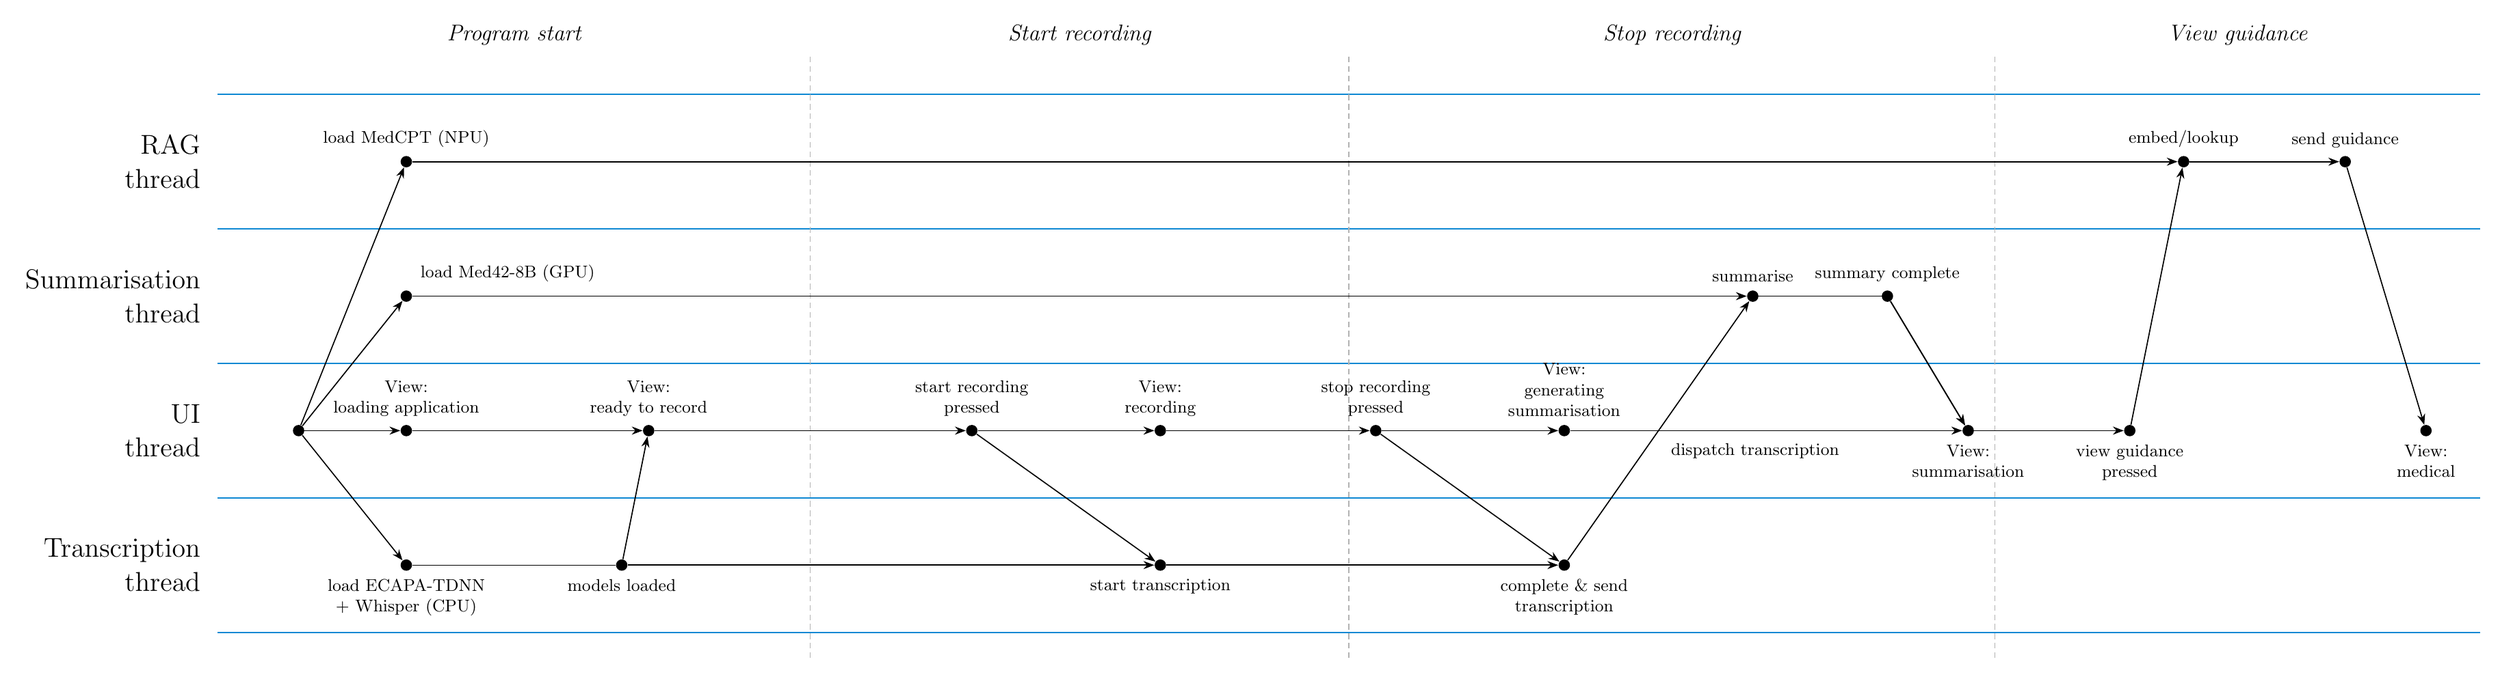
\begin{tikzpicture}[
    >=Stealth,
    event/.style={circle, fill=black, inner sep=0pt, minimum size=6pt},
    arr/.style={->, semithick},
    x=1.0cm, y=1.0cm,
]

%% Lane y-coordinates (centre of each 2.5-unit band)
\def\yRAG{8.75}
\def\ySumm{6.25}
\def\yUI{3.75}
\def\yTrans{1.25}

%% Lane boundary lines  (total width ~42)
\foreach \y in {0, 2.5, 5, 7.5, 10}
    \draw[cyan!70!blue, thick] (0, \y) -- (42.0, \y);

%% Lane labels
\node[anchor=east, font=\Large, align=right] at (-0.2, \yRAG)   {RAG\\thread};
\node[anchor=east, font=\Large, align=right] at (-0.2, \ySumm)  {Summarisation\\thread};
\node[anchor=east, font=\Large, align=right] at (-0.2, \yUI)    {UI\\thread};
\node[anchor=east, font=\Large, align=right] at (-0.2, \yTrans) {Transcription\\thread};

%% Phase separator lines
\foreach \x in {11.0, 21.0, 33.0}
    \draw[densely dashed, gray!60] (\x, 10.7) -- (\x, -0.5);

%% Phase labels
\node[font=\large\itshape] at (5.5,  11.1) {Program start};
\node[font=\large\itshape] at (16.0, 11.1) {Start recording};
\node[font=\large\itshape] at (27.0, 11.1) {Stop recording};
\node[font=\large\itshape] at (37.5, 11.1) {View guidance};

%%====================================================================
%% PHASE 1 — Program start: UI spawns the three worker threads
%%====================================================================

\node[event] (U0)  at (1.5, \yUI)    {};

%% UI → RAG
\node[event] (R0)  at (3.5, \yRAG)   {};
\node[font=\small, above=4pt] at (R0) {load MedCPT (NPU)};
\draw[arr] (U0) -- (R0);

%% UI → Summarisation
\node[event] (S0)  at (3.5, \ySumm)  {};
\node[font=\small, above right=4pt, align=left] at (S0) {load Med42-8B (GPU)};
\draw[arr] (U0) -- (S0);

%% UI → Transcription
\node[event] (Tr0) at (3.5, \yTrans) {};
\node[font=\small, below=4pt, align=center] at (Tr0)
    {load ECAPA-TDNN\\+ Whisper (CPU)};
\draw[arr] (U0) -- (Tr0);

%% UI → UI View
\node[event] (V_loading) at (3.5, \yUI) {};
\node[font=\small, above=4pt, align=center] at (V_loading)
    {View:\\loading application};
\draw[arr] (U0) -- (V_loading);
%% Transcription: models finished loading
\node[event] (Tr_ready) at (7.5, \yTrans) {};
\node[font=\small, below=4pt] at (Tr_ready) {models loaded};
\draw (Tr0) -- (Tr_ready);

%% Transcription → UI: signals models loaded
\node[event] (U_modload) at (8.0, \yUI) {};
\node[font=\small, above=4pt, align=center] at (U_modload) {View:\\ready to record};
\draw[arr] (Tr_ready) -- (U_modload);
\draw[arr] (V_loading) -- (U_modload);


%%====================================================================
%% PHASE 2 — Start recording
%%====================================================================

%% UI: user presses start recording → signals Transcription directly
\node[event] (U_srec) at (14.0, \yUI) {};
\node[font=\small, above=4pt, align=center] at (U_srec) {start recording\\pressed};
\draw[arr] (U_modload) -- (U_srec);

\node[event] (V_recording) at (17.5, \yUI) {};
\draw[arr] (U_srec) -- (V_recording);
\node[font=\small, above=4pt, align=center] at (V_recording) {View:\\recording};

%% Transcription: receives signal from UI, begins transcribing
\node[event] (Tr_sig) at (17.5, \yTrans) {};
\draw[arr] (U_srec) -- (Tr_sig);
\node[font=\small, below=4pt] at (Tr_sig) {start transcription};
\draw[arr] (Tr_ready) -- (Tr_sig); %% horizontal: models loaded → start transcription

%%====================================================================
%% PHASE 3 — Stop recording
%%====================================================================

%% UI: stop recording pressed → signals Transcription
\node[event] (U_stop) at (21.5, \yUI) {};
\node[font=\small, above=4pt, align=center] at (U_stop) {stop recording\\pressed};
\draw[arr] (V_recording) -- (U_stop); %% horizontal: View: recording → stop recording pressed

%% Transcription: receives stop signal, sends back accumulated buffer
\node[event] (Tr_send) at (25.0, \yTrans) {};
\draw[arr] (U_stop) -- (Tr_send);
\node[font=\small, below=4pt, align=center] at (Tr_send)
    {complete \& send\\transcription};
\draw[arr] (Tr_sig) -- (Tr_send);

%% UI: show the generating summarisation view
\node[event] (V_gensum) at (25.0, \yUI) {};
\draw[arr] (U_stop) -- (V_gensum);
\node[font=\small, above=4pt, align=center] at (V_gensum)
    {View:\\generating\\summarisation};

%% Transcription → Summ: dispatch transcription directly
\node[event] (S_stop) at (28.5, \ySumm) {};
\node[font=\small, above=4pt] at (S_stop) {summarise};
\draw[arr] (Tr_send) -- (S_stop)
    node[pos=0.5, below right=3pt, font=\small] {dispatch transcription};
\draw[arr] (S0) -- (S_stop); %% horizontal: load Med42-8B → summarise

%% Summ: summarisation complete
\node[event] (S_summ) at (31.0, \ySumm) {};
\node[font=\small, above=4pt] at (S_summ) {summary complete};
\draw (S_stop) -- (S_summ);

%% Summ → UI: sends summary back to UI
\node[event] (U_recv) at (32.5, \yUI) {};
\node[font=\small, below=4pt, align=center] at (U_recv) {View:\\summarisation};
\draw[arr] (S_summ) -- (U_recv);

%% V_gensum → U_recv: UI transitions directly to summarisation view
\draw[arr] (V_gensum) -- (U_recv);

%%====================================================================
%% PHASE 4 — View guidance
%%====================================================================

%% UI: user presses view guidance → goes directly to RAG
\node[event] (U_view) at (35.5, \yUI) {};
\node[font=\small, below=4pt, align=center] at (U_view)
    {view guidance\\pressed};
\draw[arr] (U_recv) -- (U_view);
\draw[arr] (S_summ) -- (U_recv);

%% RAG: receives request directly from UI
\node[event] (R_embed) at (36.5, \yRAG) {};
\node[font=\small, above=4pt] at (R_embed) {embed/lookup};
\draw[arr] (U_view) -- (R_embed);
\draw[arr] (R0) -- (R_embed); %% horizontal: load MedCPT → embed/lookup

%% RAG: performs lookup, result ready
\node[event] (R_done) at (39.5, \yRAG) {};
\node[font=\small, above=4pt] at (R_done) {send guidance};
\draw[arr] (R_embed) -- (R_done);

%% RAG → UI: returns found guidance
\node[event] (U_done) at (41.0, \yUI) {};
\node[font=\small, below=4pt, align=center] at (U_done) {View:\\medical };
\draw[arr] (R_done) -- (U_done);

\end{tikzpicture}%
}
\caption{Concurrency diagram illustrating thread interactions across the four phases of the application lifecycle.}
\label{fig:concurrency-diagram}
\end{figure}
\end{landscape}


This threading model also maps naturally onto the heterogeneous compute resources of the Intel AIPC with the transcription and diarisation models running on the CPU, the summarisation model running on the GPU, and the embeddings model running on NPU.

\subsection{Class Overview}
Figure~\ref{fig:uml_brief} illustrates the high-level object-oriented architecture of the application, demonstrating how the concurrent threads detailed in the previous section map to specific C++ classes. The architecture follows a modular approach, orchestrated by the \texttt{MainWindow} class executing on the UI thread. 

The architecture is divided into the 4 main pipelines required to handle transcription, summary, RAG and UI orchestration. 
\begin{itemize}
    \item \textbf{Audio-Transcription Pipeline (Pink, Yellow and Orange):} This pipeline handles all recording, transcription and components. The interactions within the pipeline are as follows:
    \begin{itemize}
        \item \textbf{Audio Recording and Processing (Orange)}: The \texttt{AudioRecorder} class handles all audio recording, generating an \texttt{AudioStructure} containing 30 second chunks of audio data and additional metadata required for transcription and diarisation. Every 30 seconds, the UI orchestrator thread signals for this \texttt{AudioStructure} to be published into the \texttt{AudioTranscriptionBridge}.
        \item \textbf{Audio Transcription Bridge (Yellow)}: A thread safe buffer holding the previous and next 30 seconds of audio, preventing transcription from blocking audio recording.
        \item \textbf{TranscriptionEngine (Pink)}: Subscribes to the \texttt{AudioTranscriptionBridge} to consume 30 second chunks of audio,  handling transcription then diarisation using the \texttt{DoctorEmbedding}, then appen    ding the diarised transcript to the full transcript within the class.
    \end{itemize}
    \item \textbf{SummarisationEngine (Green)}: A class to handle all summarisation, receiving a transcript and generating a summary, and signalling to the \texttt{MainWindow} once complete. This class also sends a signal to the \texttt{MainWindow} indicating that the model has loaded in case the conversation finishes first.
    \item \textbf{RAG (Pale):} Document chunking, vector indexing, and SQLite database interactions are isolated within the \texttt{GuidelineIndexer} and \texttt{GuidelineRAG} classes, returning the \texttt{GuidelineResult} to the \texttt{MainWindow} to be displayed.
    \item \textbf{UI and Orchestration (Blue)}: Controls all threads, their lifetimes and signals for the start and end of the recording pipeline, start of summarisation, and start of fetching guidelines. The \texttt{MainWindow} class is broken into several sub-classes for each UI component, which acts as a controller for their corresponding models.
\end{itemize}

Although the UI class controls the threading and flow of this application, the sub-class architecture (expanded on in TODO forward ref) ensures this class is not overloaded with different purposes. This architecture was chosen to separate concerns and combine the requirements for a concurrent approach with an extensible architecture. (The discussion on this architechture will be coming soon™) 

Showing a high level overview of the system (make this an intro)

\begin{figure}[H]
    \centering
    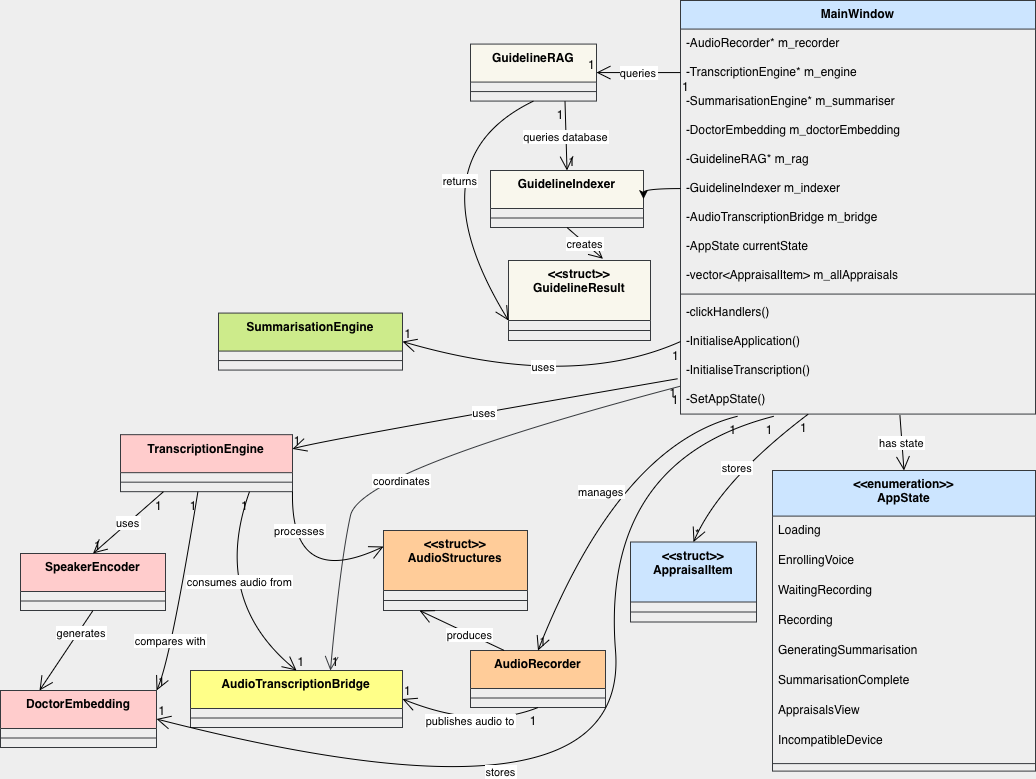
\includegraphics[width=1\linewidth]{chapters/uml_brief.drawio.png}
    \caption{This figure shows an brief overview of the classes and their interactions within the application colour coded based on the threads they occupy. All class methods and attributes except MainWindow have been removed for visual clarity}
    \label{fig:uml_brief}
\end{figure}
% TODO this has a duplicate for some reason
\section{Summarisation Engine}
\label{sec:med42testj}
\subsection{Downloading Models}
All models were downloaded and quantised using the following OpenVINO command:
\begin{verbatim}
    pip install optimum[openvino]
    optimum-cli export openvino --model <huggingface-model-name> 
                --weight-format int4 <output_directory_name>
\end{verbatim}  

\subsection{Testing Models}
To find the model that has the best trade-off between speed and accuracy, the validation set from the previous project was used to created a testing harness to evaluate each model. The \texttt{MTS-Dialog}\cite{mts-dialog} dataset contains 1,700 mock patient-doctor transcripts each with a corresponding medical summary of the conversation, with 170 samples for validation, a strong candidate for evaluating the effectiveness of each model. The dataset was created by 3 Microsoft employees to evaluate Facebook's BART-large \cite{bart} and Google's Pegasus \cite{pegasus} models fine-tuned with guided summarisation and data augmentation. 

\subsubsection{Methodology}
\label{di:test_med42}
I used the Mistral-7b, BioMistral-7b and Med42-v2-8B models for testing based on guidance from my external supervisor. Each model followed the same strategy 
\begin{enumerate}
    \item The model was quantised to int4 and was configured with \texttt{temperature=0.3} \cite{med42temp}
    \item For each validation sample, the ground truth summary, generated summary, and time taken was recorded, then saved to a CSV.
    \item BERT score was used to determine the F1, Precision, Recall metrics explained in \cite{zhang2019bertscore} to quantitatively compare the semantic accuracy of the generated summarisation against the ground truth
    \item The average time was calculated and included in the results
\end{enumerate}

This enabled a comparison between 2 key results: the inference time and accuracy. The results are as follows

\begin{figure}[H]
    \centering
    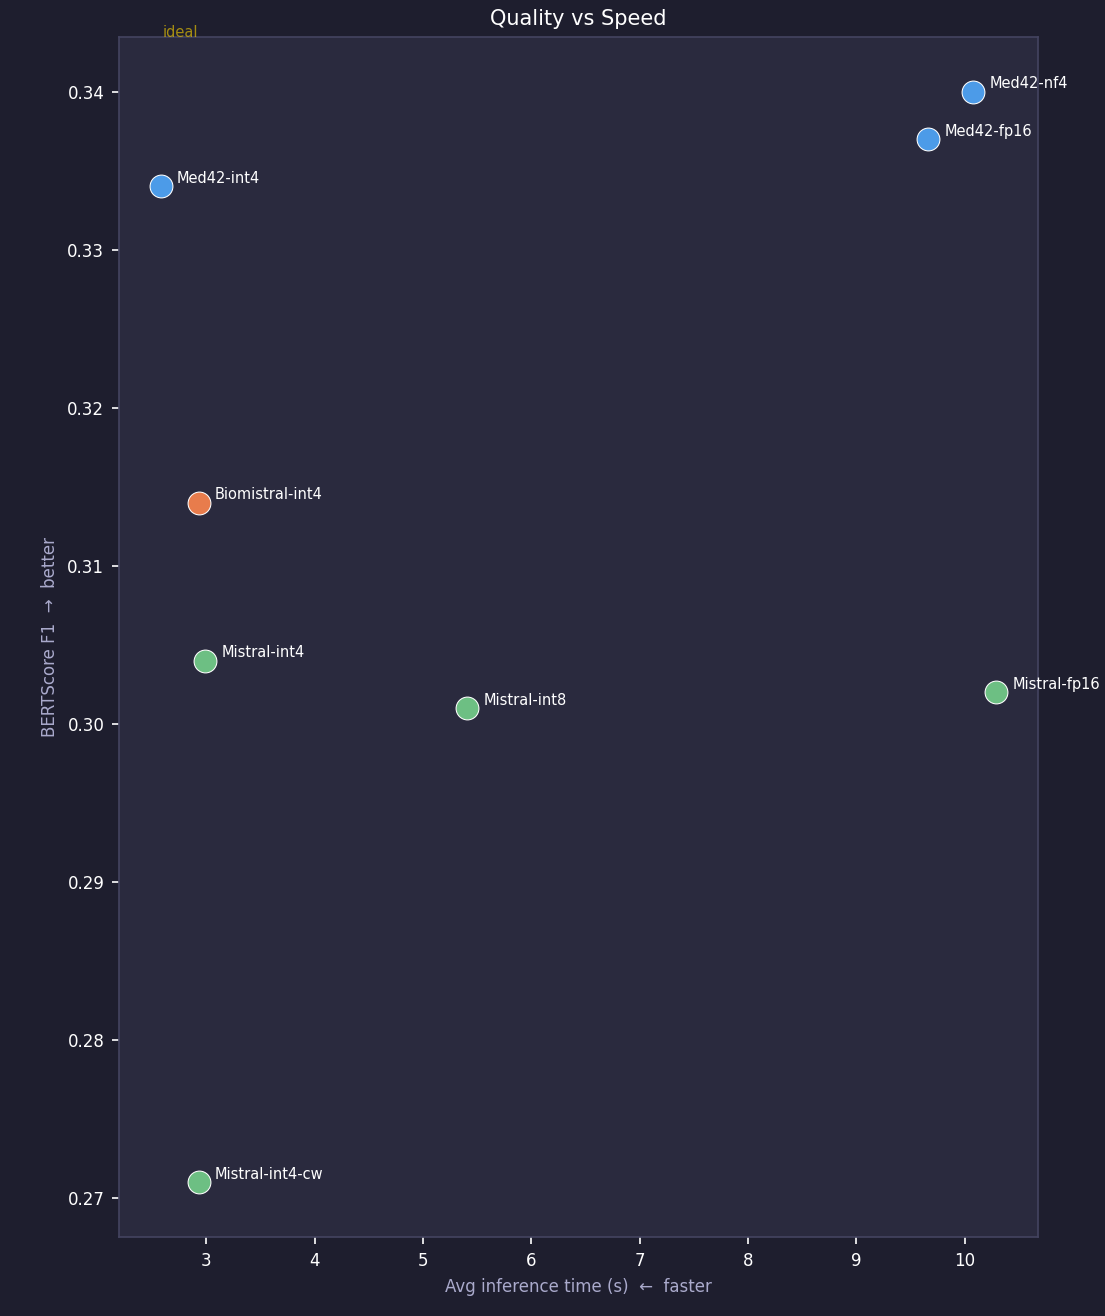
\includegraphics[width=0.75\linewidth]{model_comparison_results.png}
    \caption{A comparison between 3 models with varying quantisation levels, finding the optimal speed-accuracy tradeoff}
    \label{fig:model_comparison_results.png}
\end{figure}

We can conclude that the optimal model for this application is the Med42-v2-8B quantised to int4. As a benefit, the size of the Med42 model was reduced from 19.3GB to 4.3GB on disk.

Further testing on different devices shows the benefit of loading and running the model on the more powerful GPU compared to the NPU, resulting in the GPU being chosen for this component
\begin{figure}[htbp]
    \centering
    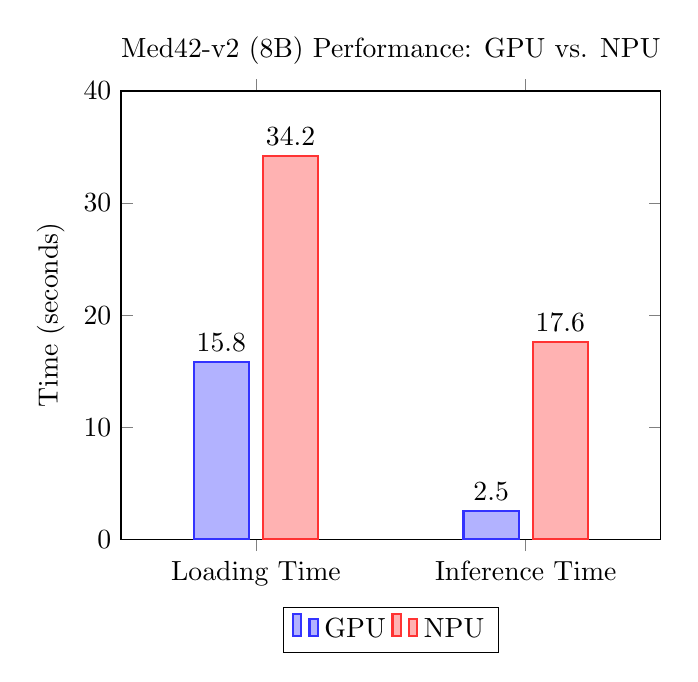
\begin{tikzpicture}
        \begin{axis}[
            ybar=5pt, % Space between the bars in a group
            bar width=20pt, % Width of the bars
            enlarge x limits=0.5, % Padding on the left and right of the chart
            legend style={at={(0.5,-0.15)}, anchor=north, legend columns=-1},
            ylabel={Time (seconds)},
            symbolic x coords={Loading Time, Inference Time}, % Swapped to be the main categories
            xtick=data,
            nodes near coords, % Displays the exact values above the bars
            nodes near coords align={vertical},
            ymin=0, ymax=40, % Normalized the height to fit the new max value (34.2)
            title={Med42-v2 (8B) Performance: GPU vs. NPU}
        ]
        
        % GPU Data (Loading, then Inference)
        \addplot[fill=blue!30, draw=blue!80, thick] coordinates {(Loading Time, 15.8) (Inference Time, 2.5)};
        
        % NPU Data (Loading, then Inference)
        \addplot[fill=red!30, draw=red!80, thick] coordinates {(Loading Time, 34.2) (Inference Time, 17.6)};
        
        \legend{GPU, NPU} % Legend now represents the hardware
        \end{axis}
    \end{tikzpicture}
    \caption{Comparison of loading and inference times for the Med42-v2 8B parameter model running on a GPU versus an NPU.}
    \label{fig:gpu_npu_performance}
\end{figure}


\subsection{Design}
\subsubsection{Concurrency}
The Med42 model requiring 20 seconds to load presents a concurrency constraint. Simply loading this model on the UI thread would cause unacceptable UI latency, therefore the following concurrency design was followed:

\begin{itemize}
    \item At program launch, a background initialisation thread is spawned to load the transcription model
    \item Once the transcription model is ready, this thread launches the Med42 summarisation model asynchronously via \texttt{std::async}, storing the result handle in a shared \texttt{std::future} member (\texttt{m\_summariserLoadFuture})
    \item An atomic boolean flag \texttt{m\_isSummariserReady} is shared between threads and set to \texttt{true} inside the async task once loading completes
    \item When the user starts recording, a separate processing thread is spawned and detached, which calls \texttt{ProcessLoop()} blocking until recording stops
    \item Once recording completes, the processing thread inspects \texttt{m\_isSummariserReady}
    \item If the model has already loaded (the common case where transcription takes longer than 20 seconds), the processing thread proceeds immediately to summary generation
    \item If the model has not yet loaded, the processing thread blocks by calling \texttt{m\_summariserLoadFuture.wait()} until the async loading task completes
    \item Once the summary is generated, the result is marshalled back to the UI thread via \texttt{DispatcherQueue().TryEnqueue()} to display
\end{itemize}

This design handles the race condition where the model has not finished loading but a transcription result arrives. Using \texttt{std::async} and \texttt{std::future} over a raw \texttt{std::thread} is preferred here because \texttt{std::future} provides a first-class blocking synchronisation primitive. The processing thread can call \texttt{wait()} directly on the future without requiring a manually managed \texttt{std::promise} or condition variable, resulting in cleaner synchronisation code.

\subsubsection{Prompting}
The effectiveness of an LLM response is highly linked to the prompt length and detail. Although pre-trained on medical textbooks and guidance, the prompt must still guide the LLM to remove any unecessary conversation and summarise only the medical facts stated to provide a history of present illness summarisation. A consultation with Dr. Tazeen Ahmed determined what was required of the summarisation resulting in the following requirements:
\begin{itemize}
    \item Facts and events must be attributed to "the doctor" or "the patient" with dates in the format DD/MM/YYYY
    \item History must be presented chronologically including onset, duration and character of pain
    \item Specific causes of injury, character of pain, aggravating factors, prior treatments and recent exacerbations must be reported
\end{itemize}

\subsection{Implementation}
The implementation is found in \texttt{SummarisationEngine.cpp}, which wraps the OpenVINO LLM pipeline with \texttt{loadModel()} and \texttt{generateFromTranscription()}

\subsubsection{Model Loading at Launch}
To launch the future from the transcription processing thread, the following implementation was chosen
\begin{verbatim}
m_summariserLoadFuture = std::async(std::launch::async, [this]() {
    try {
        m_summariser->loadModel();
        m_isSummariserReady = true;
    }
    catch (...) {
        MainWindow::SetAppState(AppState::IncompatibleDevice);
    }
});
\end{verbatim}

\texttt{std::launch::async} ensures a real OS thread is spawned. The returned \texttt{std::future<void>} is stored in the \texttt{MainWindow} member \texttt{m\_summariserLoadFuture} blocking summarisation until the task completes preventing the transcription pipeline triggering a summarisation inference before the model loads

Once loaded, the \texttt{std::atomic<bool> m\_isSummariserReady} flag is set to \texttt{true}. Should \texttt{loadModel()} throw when loading, the exception is caught and the application is moved to an \texttt{IncompatibleDevice} error state. Although the \texttt{catch} handles all error types, the only possible error when loading is a device is too little RAM or a non-Intel GPU.

\subsubsection{Waiting for the Model at Summary Time}
Once a final transcript is available, the processing thread must ensure the model is ready before calling \texttt{generateTranscription()}. It does this in two steps:

\begin{verbatim}
if (!m_isSummariserReady) {
    if (m_summariserLoadFuture.valid())
        m_summariserLoadFuture.wait();
}
\end{verbatim}

First, the atomic flag \texttt{m\_isSummariserReady} is checked. Because \texttt{std::atomic} reads are lock-free, this check is extremely cheap and covers the common case where a typical consultation lasts several minutes, well beyond the 20-second load time, so the model will almost always already be ready. If it is, execution proceeds immediately with no synchronisation overhead.

If the flag is still \texttt{false}, the thread falls through to \texttt{m\_summariserLoadFuture.wait()}. The \texttt{.valid()} guard is necessary because a default-constructed \texttt{std::future} has no associated state; calling \texttt{.wait()} on it would be undefined behaviour. \texttt{.wait()} then puts the processing thread to sleep, with no busy-waiting, until the OS wakes it once \texttt{loadModel()} returns. Critically, the UI thread is never involved in any of this waiting.

\subsubsection{Generating and Returning the Summary}
With the model guaranteed to be loaded, \texttt{generateFromTranscription()} is called synchronously on the processing thread. Once the summary string is returned, \texttt{DispatcherQueue().TryEnqueue()} marshals the result back to the UI thread for a UI update.

\subsubsection{Prompting}
The full prompt can be found in Appendix \ref{app:prompt}



\chapter{Testing}
% Describe your testing strategy (unit, functional, acceptance testing and
% how they are carried out). How were test cases selected?
% – Examples of specific tests and how they were carried out (e.g., using
% mock objects to break dependencies). Focus on the interesting cases.
% – A summary of the test results and what coverage was achieved.
% Detailed test reports should appear in the appendix, if they add useful
% information or you want to demonstrate the kinds of tests and
% coverage achieved.
% If your project requires substantial evaluation of data and results,
% evaluation of algorithms, or other forms of testing that are not code-based,
% then adapt this chapter to suit.
% This chapter will typically be 2-4 pages in length but could be more
% depending on the depth of testing done. If you need to do a detailed
% evaluation for a more mathematical or theory-based project, then this
% chapter could well be more substantial.

\section{Strategy}
The testing strategy for this project uses requirement driven testing to systematically evaluate the system against the technical, functional and non-functional requirements. This was conducted through unit testing, end-to-end testing, performance/ accuracy testing and user acceptance testing in iterative stages through the development process. A test execution matrix was created based on the requirements to ensure all requirements map to a quantifiable test case.

\section{Functional Testing}
Functional testing evaluates the application's ability to execute its core workflows and manage data correctly. This is conducted with unit tests for individual components and pipelines using Visual Studio's integrated test runner. The \texttt{gtest} library was chosen due to the integration within the Visual Studio environment allowing for quick configuration and running of the tests. When creating the unit tests for the first prototype of the application (transcription/summarisation pipeline), the architecture for the program prevented mocking external libraries. All external library and model calls were extracted to an interface to allow for a seam to provide a secure entry into the class. The tests then implement a mock interface to inject into the function for testing. The resulting design required minimal code change and no functionality change while allowing for proper mocking of back-end functionalities. An example is shown below.

\begin{verbatim}
GuidelineRAG.cpp
// extract external calls to an interface
struct GuidelineRAG::Impl {
    ov::Core core;
    ov::CompiledModel model;
    ov::InferRequest request;
    ov::genai::Tokenizer tokenizer;

    hnswlib::L2Space* space = nullptr;
    hnswlib::HierarchicalNSW<float>* index = nullptr;

    sqlite3* db = nullptr;
    int embeddingDim = 768;

    Impl(const std::filesystem::path& tokenizerPath)
        : tokenizer(tokenizerPath) {}

    ~Impl() {
        if (index) delete index;
        if (space) delete space;
        if (db) sqlite3_close(db);
    }
};

// inject the mock interface
void GuidelineRAG::SetBackendForTesting(std::shared_ptr<IGuidelineRAGBackend> backend) {
    m_testBackend = std::move(backend);
}

// an example method where we check if a mocked interface has been injected and run the method
void GuidelineRAG::Initialize(
        const std::filesystem::path& modelBasePath, 
        const std::filesystem::path& dataPath) {
    if (m_testBackend) {
        m_testBackend->Initialize(modelBasePath, dataPath);
        return;
    }
    ...
BackendTests.cpp
// an example test case
// Verifies initialize delegation through interface seam. 
TEST(GuidelineRAG, UsesInjectedBackendForInitialize) { 
    // an empty interface works for this case since no external calls were made
    GuidelineRAG rag; 
    auto backend=std::make_shared<FakeRagBackend>(); 
    rag.SetBackendForTesting(backend);
    rag.Initialize("C:\\m","C:\\d"); EXPECT_TRUE(backend->initialized);
}
\end{verbatim}

This strategy was used throughout the program, allowing for the creation of mock classes for robust unit testing. The full list of unit tests are in the appendix \ref{app:unittest}

\begin{figure}[H]
    \centering
    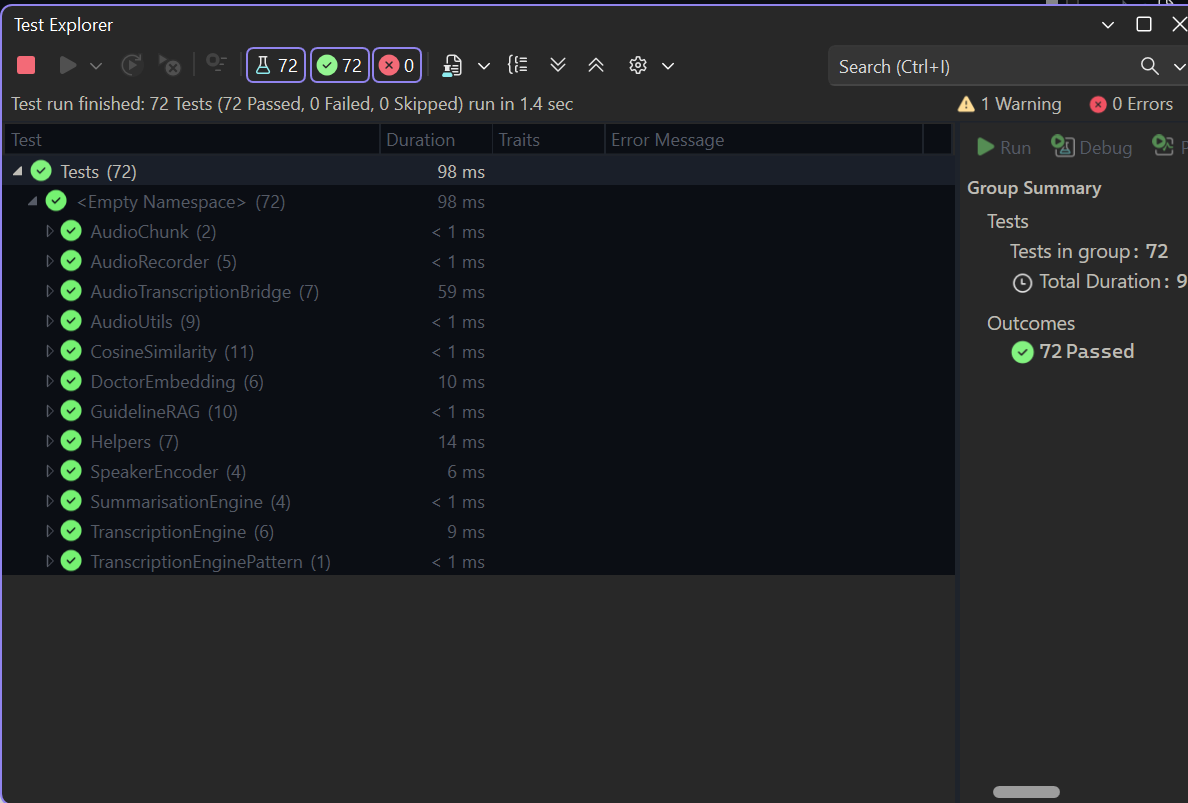
\includegraphics[width=0.5\linewidth]{unittest.png}
    \caption{All 72 unit tests passing within the Visual Studio Text Explorer}
    \label{fig:placeholder}
\end{figure}

\section{Performance Testing}
Performance testing was conducted to verify that the application meets teh latency and responsiveness constraints defined in requirements NF1-4. All tests were executed on the target Intel AI PC.

\begin{table}[H]
\centering
\begin{tabular}{|l|p{6cm}|l|l|}
\hline
\textbf{Req ID} & \textbf{Performance Metric} & \textbf{Target Constraint} & \textbf{Observed Result} \\ \hline
NF1 & Application startup and complete ML model loading into memory & $< 60$ seconds & Med42: $20$s, other models: $4$s \\ \hline
NF2 & Summary generation completion after a 15-minute consultation & $< 90$ seconds & $73$ seconds \\ \hline
NF3 & Semantic search and guidance retrieval over uploaded documents & $< 3$ seconds & $< 1$ second \\ \hline
NF4 & UI Responsiveness during heavy background processing & No freezing/hangs & Completely fluid \\ \hline
\end{tabular}
\caption{Summary of performance testing results against non-functional requirements.}
\label{tab:performance_results}
\end{table}


\subsubsection{Summarisation Inference}
To test the NF2 requirement, a 15 minute mock conversation was conducted with a friend. By recording the time taken for the conversation and inference, we found the result of around 73 seconds for a 15 minute conversation. This can be confirmed by our model benchmarks. During model selection, the longest conversation sample (228 words) required 392 tokens and was inferenced in 6.65 seconds by the Med42-8b int4 model resulting in 58.9 tokens/second or roughly 34 words/second. Extrapolating this to a 15 minute, 2000 word consultation, results in a predicted 58 second inference time.

\subsubsection{Retrieval Latency (NF3)}
This requirement was tested by uploading 3 medical PDFs and pressing "view guidance". On an average of 10 runs, the time taken between pressing "view guidance" and the UI displaying the highlighted guidance within the PDF averaged 2 seconds.

\subsubsection{UI Responsiveness (NF4)}
Throughout all UI testing, the user interface remained responsive with no noticeable delay

\subsection{Accuracy Testing}
\subsubsection{Summarisation}
After selecting Med42 as our summarisation model, the LLM testing framework (TODO link) was re-ran with the \texttt{rescale\_with\_baseline\=False} to provide an individual benchmark over a comparative benchmark. The results provided in \ref{fig:med42_benchmark} demonstrating it is fit for purpose with a precision score of 88\%.

\begin{figure}[H]
    \centering
    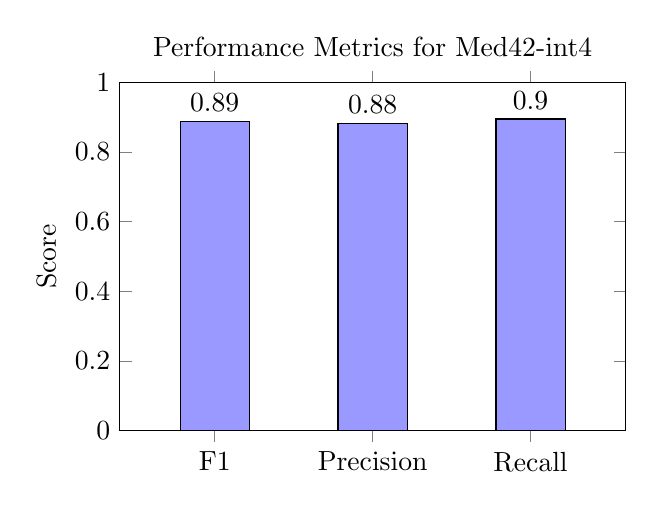
\begin{tikzpicture}
        \begin{axis}[
            ybar,
            title={Performance Metrics for Med42-int4},
            ylabel={Score},
            symbolic x coords={F1, Precision, Recall},
            xtick=data,
            ymin=0.0, ymax=1.0, % Zoomed in slightly to show the differences better
            nodes near coords, % Displays the numbers on top of the bars
            nodes near coords align={vertical},
            bar width=25pt,
            enlarge x limits=0.3, % Adds space on the left and right sides
            width=8cm,
            height=6cm
        ]
        
        \addplot[fill=blue!40] coordinates {
            (F1, 0.888) 
            (Precision, 0.882) 
            (Recall, 0.895)
        };
        
        \end{axis}
    \end{tikzpicture}
    \label{fig:med42_benchmark}
    \caption{Evaluation metrics for the Med42-int4 model.}
\end{figure}

\subsubsection{Transcription}
The accuracy of the transcription in this clinical setting was tested on medical terminology. A glossary of medical terminology published by the European Medicines Agency \cite{ema_medical_terms_simplifier} was used as the ground truth set. This was conducted by running the application and speaking 4 randomly selected words for each starting letter of the alphabet. Once completed, the transcription was viewed and compared against the glossary. To analyse these results, each word was placed into a category of correct, minor inaccuracy (punctuation or American English) and major inaccuracy.

\begin{table}[htbp]
\centering
\begin{tabular}{|c|c|c|c|}
\hline
\textbf{Count} & \textbf{Correct} & \textbf{Inaccuracy} & \textbf{Incorrect} \\
\hline
104 & 93 & 8 & 3 \\
\hline
\end{tabular}
\caption{Transcription results with Whisper-Medium on 104 medical terminology samples}
\label{tab:results}
\end{table}

Generally, the transcription model has a large enough vocabulary to accurately transcribe medical terminology. Common inaccuracies involve incorrect hyphens, American English spelling, and incorrect capitalisation. The incorrectly transcribed words included syncope, fissure and tophi miss-transcribed to sync up, Fisher and trophy. This is likely due to the transcribed words having higher weights within the model due to their popularity compared to the niche medical terminology. Overall an 93\% accuracy on medical terminology is acceptable, especially since the summarisation can infer context. The full results can be examined in Appendix \ref{app:testing_transcription_results}.

\subsubsection{Diarisation}
The speaker diarisation model provides a score from 0-1 on how likely the person speaking is the doctor for a given audio chunk. Empirical testing was conducted to determine what the threshold value should be to decide if the doctor was speaking or someone else. By encoding the doctor as person myself, 1 minute of audio was captured each for myself and a friend reading the introduction to this dissertation. The results showed the average doctor score to be 0.76, with the patient score as 0.54, leading to the threshold value set at 0.7.

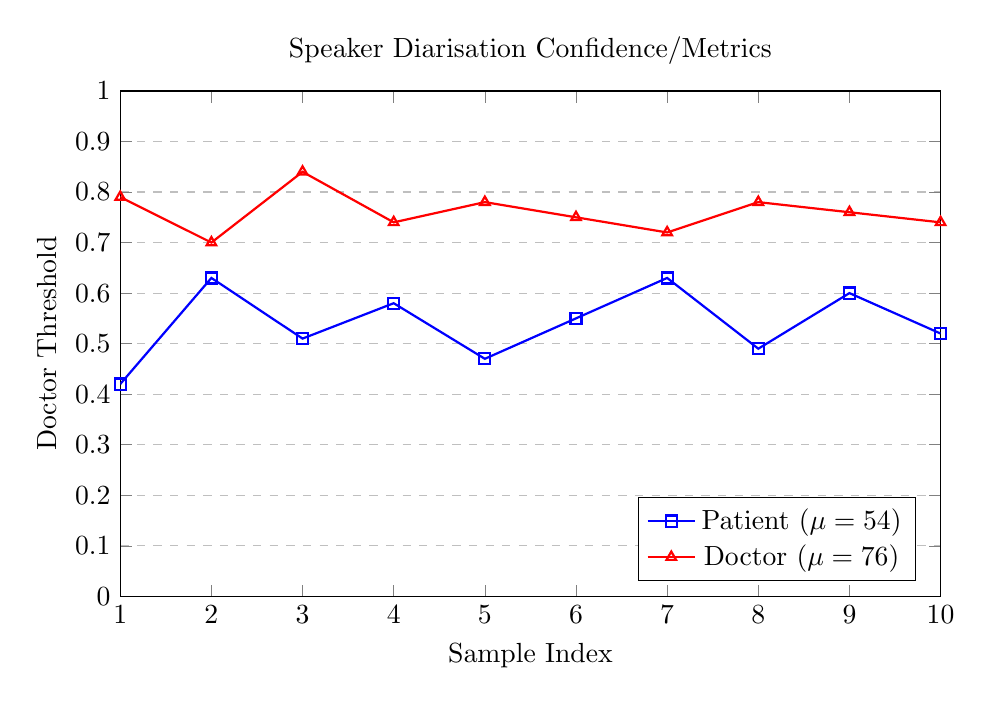
\begin{tikzpicture}
\begin{axis}[
    title={Speaker Diarisation Confidence/Metrics},
    xlabel={Sample Index},
    ylabel={Doctor Threshold},
    xmin=1, xmax=10,
    ymin=0, ymax=1, 
    xtick={1,2,3,4,5,6,7,8,9,10},
    ytick={0, 0.1, 0.2, 0.3, 0.4, 0.5, 0.6, 0.7, 0.8, 0.9, 1.0},
    legend pos=south east,
    ymajorgrids=true,
    grid style=dashed,
    width=12cm,
    height=8cm
]

\addplot[
    color=blue,
    mark=square,
    thick
]
coordinates {
    (1, 0.42)
    (2, 0.63)
    (3, 0.51)
    (4, 0.58)
    (5, 0.47)
    (6, 0.55)
    (7, 0.63)
    (8, 0.49)
    (9, 0.60)
    (10, 0.52)
};
\addlegendentry{Patient ($\mu = 54$)}

\addplot[
    color=red,
    mark=triangle,
    thick
]
coordinates {
    (1, 0.79)
    (2, 0.70)
    (3, 0.84)
    (4, 0.74)
    (5, 0.78)
    (6, 0.75)
    (7, 0.72)
    (8, 0.78)
    (9, 0.76)
    (10, 0.74)
};
\addlegendentry{Doctor ($\mu = 76$)}

\end{axis}
\end{tikzpicture}

The full results can be examined here \ref{app:speaker_diarisation_results}

\subsubsection{Guidelines Retrieval}
Due to the custom retrieval pipeline implementation, testing with a ground truth PDF dataset is unfeasible. Without a found ground truth set, no quantitative testing or results can be generated. That being said, qualitative testing was completed. Generally speaking, the retrieved guidance was accurate, however was highly dependent on the specificity of the guidance PDFs uploaded. General documents laying out a disease progression or advice for trivial diseases provided little valuable insights. Very specific guidance documents were highly effective at retrieving medical guidance that is important to the conversation.

\section{UI Testing}
User interface testing began by testing every state transition in the application to ensure that the state management system was functional. Next, persistent data such as the doctor's voice embedding, appraisals and uploaded guidance was loaded, then checked for their presence after an application restart. All tests passed, while the UI stayed responsive and in the state we were expecting. A full list of test cases is in the appendix \ref{app:UI_test}

\section{User Acceptance Testing}
Throughout the project, 5 demonstrations and 2 trials of the application were conducted with Dr Atia Rafiq and Dr Tazeen Ahmed. At a UCL hosted AI conference, I trialled the application by mocking a consultation with Dr Tazeen Ahmed where she used the application as if she was conducting a real consultation. The application took no explanation on how to use and the consultation was successfully carried out resulting in a successful user acceptance test(TODO requirement). She expressed her enthusiasm with the project and commented that this application would "save her lots of time taking notes and reviewing consultations throughout the day". She further commented that the appraisals system would be "highly beneficial" for training GPs. She also provided feedback regarding the prompt, requesting the prompt to use the "the patient says" and "the doctor suggested" formats which were integrated after the event.

On a video call with Dr Atia Rafiq, I demonstrated the application. She noted that the user interface looked easy to use and had an appeasing design and that the application would be very useful to her and her trainee GPs. She added a further recommendation to create the appraisals component to allow note taking and commentary on conversations to demonstrate learning that was conducted post-consultation.





\chapter{Evaluation and Conclusion}
% A summary of what the project has achieved. Make sure that you
% address each goal set out in the Introduction chapter, to show that you
% have achieved what you claimed you would. Don’t leave any loose
% ends.
% – A critical evaluation of the results of the project (e.g., how well were
% the goals met, is the application fit for purpose, has good design and
% implementation practice been followed, was the right implementation
% technology chosen and so on).
% – Future work. How could the project be developed if you had another 6
% months. Take care to differentiate between what you have done to
% satisfy your stated project goals, and work that could be done to meet
% extended goals.
% – Wrap-up and final thoughts on your project.
\section{Achievements}
This project has completed all of the goals set out in the introduction providing evidence that this proof-of-concept is worth persuing for future development. The initial comparison between candidate medical LLMs showed Med42-v2 to have the optimal accuracy-speed tradeoff out of the candidate models, demonstrating the effectiveness of OpenVINO's model quantisation framework. A real time transcription-diarisation pipeline was implemented using the \texttt{Whisper-Medium} and \texttt{ECAPA-TDNN} models, connected to the summarisation pipeline. The appraisal entry system was created based on feedback from Dr. Atia Rafiq, and a guidelines retrieval component was realised. An iterative approach to the UI design enabled an appealing and user friendly end product, native to Windows. Finally, the application design using the orchestator and pipeline design patterns, and sub-implementations of the controllers resulted in an extensible application. 

Outside of the goals, I produced 6 demonstration videos, one of which was presented at the shard at a Dell event for Intel and NHS stakeholders. The final build of the application was presented at a an Intel sponsored HP booth at the NHS Strategy Summit on the 29th April 2026. I featured on the UCL Computer Science LinkedIn page while conducting demonstrations to healthcare professionals and presented to 50 healthcare professionals at the UCL Computer Science Showcase 2026. Finally, the application has been published through my supervisor's Motion Input Games platform and is free to download (strictly for demonstration purposes) at \url{https://www.motioninputgames.com/software/AIPC/health/Clinical-Summarisation-AI-PC_1.0.10.0_x64.msix}.

\section{Critical Evaluation of the Results}
The project was successful in demonstrating that an offline clinical documentation workflow can be implemented on Intel AI PC hardware using a combination of quantised language models, speech recognition, speaker diarisation, and local retrieval. The implemented system satisfies the intended proof-of-concept scope as it records a consultation, produces a structured summary, stores supporting data locally, and allows clinicians to attach contextual guidance and appraisal material without relying on cloud infrastructure. 

The application design followed sound software engineering principles, particularly through separation of concerns. The concurrent architecture isolated the user interface from computationally expensive inference tasks, which was important for maintaining responsiveness during a consultation. The data management approach also separated transient workflow data from persistent records such as appraisal JSON files and the SQLite database. Interface abstraction enabled the use of mock objects during testing, which improved the ability to evaluate components in isolation.

Some design decisions also introduced limitations. The choice to keep user interface state within a single \texttt{MainWindow} class, even when split across multiple translation units, was understandable for a sequential proof-of-concept but is less maintainable than a full MVVM architecture if the interface grows further. The evaluation is also stronger on functional demonstration than on formal quantitative validation. For example, this project presents evidence that the transcription and summarisation pipeline works in practice, but there is limited end-to-end measurement of consultation time saved, documentation quality, or retrieval relevance across a large dataset. Formal user acceptance testing and a clinical trial would be required to determine whether the application provides measurable benefit to GPs compared to other solutions. Furthermore, additional research into alternative models such as Whisper-Turbo or a mechanism to enable user uploaded models would be required to establish the correctness of the models chosen. As result, this project demonstrates feasibility more than clinical time saved.

The development process was generally effective, particularly where regular meetings with supervisors and clinicians helped keep the work aligned with practical requirements. However, an early assumption that NICE API access would be feasible proved incorrect. This led to redesign work later in the project and resulted in a less integrated retrieval approach based on clinician uploaded guidance documents. 

\section{Future Work}
Although the proof-of-concept met its core requirements, several important extensions remain out of scope. The most significant short-term goal would be a structured clinical evaluation. A planned trial with Dr Tazeen Ahmed at St. George's Hospital was blocked because of the March-April 2026 cyber attack, but a future study of this kind would be valuable. Measuring time saved, documentation burden, usability, and perceived accuracy during real consultations would enable a comparative study against current solutions. It would also identify where the current workflow creates friction for clinicians.

If access to the NICE API became available, a hybrid online-offline architecture could download updated guidance at controlled intervals while preserving local inference during use. This would enable more rigorous retrieval evaluation over a larger and better defined document collection.

Further feature development could also build on the existing pipeline structure. Translation was discussed during the project but remained out of scope however, adding a translation stage could improve accessibility for multilingual consultations. Additional recording functionality, such as hands-free activation, could better match how clinicians work in practice. Speech-to-text input for appraisal notes would also be a natural extension of the current transcription pipeline as suggested by Dr. Atia Rafiq.

Finally, future hardware and OpenVINO improvements may allow larger local models and longer prompts, which could improve summarisation quality. The direction of current AI PC development and potential quantisation improvements could allow larger summarisation models to be tested. Future summarisation work could also include patient-friendly explanations of diagnoses and tighter integration of retrieved guidance into the generated summary.

\section{Conclusion}
This project demonstrated that an offline, Windows-native clinical summarisation system is feasible. The final application combines local speech transcription, diarisation, summarisation, appraisal support, and retrieval of medical guidance into a coherent proof-of-concept workflow. While the evaluation does not yet establish clinical effectiveness at deployment scale, it does show that the underlying architecture and implementation are strong enough to support further development.

Personally, I learned a new programming language, development environment, packaging environment and font-end stack. This lead to lots design and planning, with many teething problems throughout the highly challenging yet enjoyable development journey. Overall, this project acts as the first building block towards offline AVT solutions for Intel and the NHS to reduce the time taken and fatigue caused by note taking and documentation within clinical consultations throughout healthcare.

\appendix

\printbibliography
% \bibliographystyle{unsrt}
% \bibliography{main}

\chapter{Requirements}
\label{app:requirements}
Requirements are organised into four categories: general requirements covering project-level constraints and deliverables, technical requirements specifying platform and hardware constraints, functional requirements describing what the application must do, and non-functional requirements specifying quality attributes the application must exhibit prioritised with the MoSCoW system. Each requirement is assigned a unique identifier for traceability.

\subsection{General Requirements}
\label{app:greq}
\begin{table}[H]
\centering
\begin{tabularx}{\textwidth}{l X}
\toprule
\textbf{ID} & \textbf{Requirement} \\
\midrule
G1 & The application must be delivered as a proof-of-concept demonstrating the feasibility of offline clinical AVT on Intel AIPC hardware. \\
G2 & The application must be publishable to the Microsoft Windows Store as an MSIX packaged application. \\
G3 & Video demonstrations and presentations must be delivered to clients and supervisors on request, tailored to the target audience and iteratively refined based on feedback. \\
G4 & Workshops and presentations at relevant events must be attended to gather feedback from healthcare professionals and promote the project. \\
G5 & The application must be designed with extensibility in mind so that future developers can extend this proof-of-concept towards an industry ready product. \\
G6 & All source code must be hosted on GitHub with a branching strategy that supports parallel feature development and rollback. \\
\bottomrule
\end{tabularx}
\caption{General requirements}
\label{tab:greq}
\end{table}

\subsection{Technical Requirements}
\label{app:treq}

\begin{table}[H]
\centering
\begin{tabularx}{\textwidth}{l X}
\toprule
\textbf{ID} & \textbf{Requirement} \\
\midrule
T1 & The front-end must be built with WinUI3 using XAML for the UI layer and C++/WinRT for the application logic. \\
T2 & The back-end inference pipeline must use Intel's OpenVINO toolkit to execute all machine learning models on-device. \\
T3 & The target hardware platform is an Intel AI PC with a minimum of 32\,GB system RAM, 18\,GB VRAM, and an integrated NPU. \\
T4 & All machine learning models must be converted to OpenVINO IR format and quantised to int4 or int8 weight precision prior to distribution. \\
T5 & The application must operate entirely offline with zero network communication to external services during all use cases. \\
T6 & The development environment must facilitate the MSIX packaging platform. \\
T7 & Pre-trained medical LLMs with no more than 10 billion parameters must be evaluated and selected to fit within the memory constraints of T3. \\
T8 & The speech-to-text model must be from the Whisper family due to OpenVINO's native \texttt{WhisperPipeline} support. \\
T9 & The application must record a conversation and process the audio stream in real time, building the transcription live during the conversation. \\
T10 & The concurrent architecture must allow all models to run simultaneously in memory to avoid loading overheads. \\
\bottomrule
\end{tabularx}
\caption{Technical requirements}
\label{tab:treq}
\end{table}

\subsection{Functional Requirements}
\label{app:freq}

Functional requirements are prioritised using the MoSCoW method. \textit{Must Have} requirements define the minimum viable product. \textit{Should Have} requirements add significant value but are not blocking. \textit{Could Have} requirements are desirable extensions that fall outside the core scope.

\subsubsection{Must Have}

\begin{table}[H]
\centering
\begin{tabularx}{\textwidth}{l X}
\toprule
\textbf{ID} & \textbf{Requirement} \\
\midrule
F1 & The user must be able to select an audio input device from any microphone connected to the laptop, including the built-in microphone as default. \\
F2 & The application must diarise the conversation in real time by labelling each transcribed segment as either \texttt{[Doctor]} or \texttt{[Patient]}, based on a pre-recorded voice embedding of the doctor. \\
F3 & The user must be able to record their voice before a consultation to generate the voice embedding used for diarisation. \\
F4 & The recorded voice embedding must be saved and encrypted locally for use in future conversation. \\
F5 & On completion of a conversation, the application must generate a clinical summary of the diarised transcript using a pre-trained medical LLM. \\
F6 & The user must be able to save the transcript and summary to a user-specified location on the local file system. \\
F7 & A default save location for summaries, transcripts and appraisal entries must be available for the user to select. \\
F8 & The relevant NICE Guidelines must be found based on the summary. \\
F9 & After summarisation, the application must retrieve and display the sections of uploaded medical guidance most relevant to the consultation summary, using a semantic search pipeline. \\
F10 & Retrieved guidance must be displayed within an embedded PDF viewer with the relevant sections visually highlighted. \\
F11 & The application must provide clear visual feedback during long-running operations (transcription, summarisation, guidance retrieval) so the user is aware of the current processing state. \\
F12 & The application must provide a responsive, intuitive Windows-native user interface suitable for clinicians with varying levels of technical proficiency. \\
F13 & A help and information section must be available to the user at all times providing necessary legal disclaimers and help for each section of the application\\
\bottomrule
\end{tabularx}
\caption{Functional requirements (Must Have)}
\label{tab:fmreq}
\end{table}

\subsubsection{Should Have}

\begin{table}[H]
\centering
\begin{tabularx}{\textwidth}{l X}
\toprule
\textbf{ID} & \textbf{Requirement} \\
\midrule
F14 & The user should be able to create appraisal entries from a completed summarisation, attaching free-text notes and tags to each entry. \\
F15 & Appraisal entries should be searchable by name and filterable by tag. \\
F16 & The user should be able to view, edit, and delete individual appraisal entries, and delete all entries at once. \\
F17 & The application should support the upload and semantic searching of non-NICE medical guidance PDFs alongside NICE guidelines. \\
\bottomrule
\end{tabularx}
\caption{Functional requirements (Should Have)}
\label{tab:fsreq}
\end{table}

\subsubsection{Could Have}

\begin{table}[H]
\centering
\begin{tabularx}{\textwidth}{l X}
\toprule
\textbf{ID} & \textbf{Requirement} \\
\midrule
F18 & Multi-lingual transcription and translation support during conversation. \\
F19 & Voice recording of post-consultation notes appended to the transcript. \\
F20 & A patient-facing plain-language summary generated alongside the clinical summary. \\
F21 & A voice-activated trigger (e.g.\ ``Hey Ambience'') to begin recording without pressing a button. \\
F22 & Integration with EPR systems to export summaries directly into patient records. \\
\bottomrule
\end{tabularx}
\caption{Functional requirements (Could Have)}
\label{tab:fcreq}
\end{table}

\subsection{Non-Functional Requirements}
\label{app:nreq}

\begin{table}[H]
\centering
\begin{tabularx}{\textwidth}{l l X}
\toprule
\textbf{ID} & \textbf{Category} & \textbf{Requirement} \\
\midrule
NF1 & Performance & The application must start and load all ML models into memory within 60 seconds of launch. \\
NF2 & Performance & Summary generation must complete within 90 seconds of the conversation ending for a consultation of up to 15 minutes. \\
NF3 & Performance & Semantic search over uploaded guidance documents must return results within 3 seconds. \\
NF4 & Performance & The UI must remain responsive (no freezing or dropped frames) during all background processing operations including recording, transcription, and summarisation. \\
NF5 & Security & The application must encrypt the doctor's voice embedding as this constitutes to biometric data\\
NF6 & Security & The application must make zero outbound network requests during operation, ensuring patient data never leaves the device. \\
NF7 & Usability & The interface must be navigable by clinicians with no prior training, using standard Windows UI conventions and clear labelling. \\
NF8 & Usability & All primary workflows (start recording, stop recording, view summary, view guidance) must be achievable within three clicks from the main screen. \\
NF9 & Reliability & The application must handle errors during model inference (e.g. incompatible device) gracefully, displaying an informative error message without crashing. \\
NF10 & Maintainability & The codebase must follow a modular architecture with separation between UI, data processing and model inference components to enable future extensions\\
NF11 & Portability & The application must run on any Intel AIPC meeting the hardware specification in T3 without requiring manual driver or dependency installation by the end user. \\
\bottomrule
\end{tabularx}
\caption{Non-functional requirements}
\label{tab:nreq}
\end{table}
\chapter{Requirements Traceability Matrix}
\label{app:requirements_traceability}

Table~\ref{tab:rtm} maps each requirement to the design decisions and system components that address it. This provides forward traceability from requirements to design, ensuring every requirement has a corresponding implementation strategy and no design decision exists without a motivating requirement.

\begin{longtable}{l p{5.2cm} p{6.8cm}}
\toprule
\textbf{Req.} & \textbf{Design Decision} & \textbf{Realising Component(s)} \\
\midrule
\endfirsthead
\toprule
\textbf{Req.} & \textbf{Design Decision} & \textbf{Realising Component(s)} \\
\midrule
\endhead
\midrule
\multicolumn{3}{r}{\textit{Continued on next page}} \\
\bottomrule
\endfoot
\bottomrule
\caption{Requirements traceability matrix mapping requirements to design decisions and components.}
\label{tab:rtm}
\endlastfoot
G1 & Proof-of-concept scope; offline-first architecture & Full application pipeline \\
G2, T6 & MSIX packaging with WinUI3 & Visual Studio MSIX project template \\
G5 & Modular architecture with separated concerns & Layered component structure (UI, inference, data) \\
G6 & Git branching strategy & GitHub repository with feature branches \\
\midrule
T1 & Native Windows front-end & WinUI3 XAML views, C++/WinRT click and state handlers \\
T2 & On-device inference engine & OpenVINO C++ API \\
T3 & Hardware based model selection & Int4/int8 quantised models sized for 32\,GB RAM, 18\,GB VRAM target device \\
T4 & Pre-distribution quantisation & OpenVINO \texttt{optimum-cli} conversion \\
T5 & No network calls; all models bundled locally & Bundled model weights in MSIX package; SQLite in-process database; HNSWLib in-memory index \\
T7 & Sub-10B parameter constraint & Med42-8B selected after benchmarking \\
T8 & Whisper family constraint & Whisper-Medium via OpenVINO \\
T10 & Concurrency strategy \autoref{fig:concurrency-diagram} & Each model (except diarisation and translation) runs on different threads and devices\\
\midrule
F1 & Audio device enumeration & MiniAudio device listing API \\
F2, T9 & Streaming audio capture with real-time transcription & Audio capture thread $\rightarrow$ shared buffer $\rightarrow$ transcription thread running Whisper-Medium and ECAPA-TDNN \\
F3 & Cosine similarity of voice embeddings & ECAPA-TDNN model comparing segment embeddings against doctor embedding \\
F4 & Voice enrolment workflow & Dedicated UI dialog, ECAPA-TDNN embedding computation, encrypted local storage of embedding \\
F5 & Post-conversation LLM inference & Summarisation thread running Med42-8B on GPU via OpenVINO \\
F6 & File save dialog & Windows native file picker via WinRT API \\
F7, F8 & Document management UI & Guidance view with upload/delete controls, SQLite metadata table \\
F9 & Semantic search pipeline & MedCPT embedding of summary $\rightarrow$ HNSWLib ANN query against guidance embeddings \\
F10 & Embedded PDF viewer with highlighting & MuPDF rendering with bounding-box overlays \\
F11 & Async processing with UI feedback & Progress indicators and status text updated from background threads via WinUI3 dispatcher \\
F12 & Three-view navigation structure & NavigationView with Recording, Appraisals, and Guidance pages \\
F13 & Persistent UI help/info buttons & Help/info flyout\\
F14-F16 & Appraisal CRUD with tagging & JSON appraisals storage, tag filtering and sorting, dialog-based CRUD modifications \\
F17 & Generic PDF support in RAG & MedCPT chunking and embedding pipeline applied to any uploaded PDF\\
\midrule
NF1 & Real time transcription & Dedicated transcription threaded pipeline\\
NF2 & Summary within 90\,s & Med42-8B int4 on GPU; prompt engineering to constrain output length \\
NF3 & Guidance retrieval within 3\,s & Pre-indexed HNSWLib graph; MedCPT embedding computation \\
NF4 & UI never blocks & Multi-threaded architecture, dispatcher-based UI updates \\
NF5 & Encryption at rest & Encrypted voice embedding file \\
NF6 & Zero outbound network traffic & No HTTP/socket calls in codebase\\
NF7--8 & Intuitive three-click workflows & Standard WinUI3 controls, NavigationView, minimal dialog depth \\
NF9 & Graceful error handling & Try-catch around OpenVINO inference calls, user-facing error dialogs \\
NF10 & Modular codebase & Separated UI layer, audio module, inference module, data-access module \\
NF11 & No manual dependency install & All dependencies bundled in MSIX package \\
\end{longtable}
\chapter{Testing Speaker Diarisation Results}
\label{app:speaker_diarisation_results}
\subsection{Doctor Transcript}
\noindent
{[Doctor 0.79]} This research investigates the application of on-device machine learning and clinical administration \newline
{[Doctor 0.70]} through the development of an offline Windows application. As a proof of concept, \newline
{[Doctor 0.84]} the primary objective is to evaluate the feasibility of a native Windows application \newline
{[Doctor 0.74]} running on an Intel AI PC to autonomously record consultations, transcribe audio, \newline
{[Doctor 0.78]} perform speaker diarisation, generate clinical summaries, and retrieve medical guidance within an entirely offline environment. \newline
{[Doctor 0.75]} While existing cloud-based systems such as TORTUS AI, Heidi Health, and Nuance DAX Copilot \newline
{[Doctor 0.72]} highlight the utility of automated clinical documentation within healthcare, \newline
{[Doctor 0.78]} they rely on networked deployment, extensive integration, and external data processing. \newline
{[Doctor 0.76]} In the context of the National Health Service, these dependencies introduce significant data governance and infrastructural challenges. \newline
{[Doctor 0.74]} Consequently, developing an offline proof of concept provides a mechanism to evaluate an alternative deployment architecture designed to address these specific operational constraints.

\vspace{1em}

\subsection*{Patient Transcript}
\noindent
{[Patient 0.42]} This research investigates the application of on-device machine learning \newline
{[Patient 0.63]} and clinical administration through the development of an offline Windows application. \newline
{[Patient 0.51]} As a proof of concept, the primary objective is to evaluate the feasibility \newline
{[Patient 0.58]} of a native Windows application running on an Intel AI PC to autonomously \newline
{[Patient 0.47]} record consultations, transcribe audio, perform speaker diarisation, generate clinical summaries, \newline
{[Patient 0.55]} and retrieve medical guidance within an entirely offline environment. While existing cloud-based \newline
{[Patient 0.63]} systems such as TORTUS AI, Heidi Health, and Nuance DAX Copilot highlight the utility \newline
{[Patient 0.49]} of automated clinical documentation within healthcare, they rely on networked deployment, extensive integration, and external data processing. \newline
{[Patient 0.60]} In the context of the National Health Service, these dependencies introduce significant data governance \newline
{[Patient 0.52]} and infrastructural challenges. Consequently, developing an offline proof of concept provides a mechanism to evaluate an alternative deployment architecture designed to address these specific operational constraints.
\chapter{Code Listings}
\label{app:code_listings}

\section{Summarisation Engine - Prompt}
\label{app:generate_transcription}

\begin{verbatim}
// prompt med42 with transcript to create summary
std::string SummarisationEngine::generateFromTranscription(std::string transcript) {
    std::string systemPrompt =
        "<|system|>\n"
        "You are an expert Clinical Medical Summariser for the NHS in England. Your task is to document a formal History of Present Illness (HPI) based on the doctor-patient transcript.\n"
        "Rules for Documentation:\n"
        "1. **Style**: Write in a formal, objective clinical style (Third Person). Do not tell a story.\n"
        "2. **Attribution**: Attribute facts to the patient (e.g., use 'The patient stated...', 'She reports...', 'Patient notes...').\n"
        "3. **Detail**: Capture specific causes of injury, specific dates (convert spoken dates to DD/MM/YYYY), and specific names of providers if mentioned.\n"
        "4. **Chronology**: Present the history chronologically, starting with the initial onset/injury.\n"
        "5. **Content**: Include onset, duration, character of pain, aggravating factors, prior treatments, and recent exacerbations.\n"
        "\n"
        "Output Requirements:\n"
        "- Correct minor grammar mistakes but keep medical facts exact.\n"
        "- Output ONLY the final clinical note text. Do not chat or add introductory text.\n"
        "- Keep summarisation as brief as possible, ignore non-medical conversation, do not make assumptions on anything not explicitly mentioned in the transcript\n"
        "- Do not infer dates or activities not present in the text.\n"
        "- Do not provide any medical guidance";

    std::string userPrompt =
        "<|user|>\n"
        "TRANSCRIPT:\n" + transcript + "\n"
        "<|assistant|>\n"
        "SUMMARISATION: \n";

    std::string fullPrompt = systemPrompt + userPrompt;

    ov::genai::GenerationConfig config;
    config.max_new_tokens = 1024; 
    config.temperature = 0.2f;   

    ov::genai::DecodedResults res = m_model->generate(fullPrompt, config);

    return res.texts[0];
}
\end{verbatim}
\chapter{Test Execution Matrix}
\label{app:test_matrix}
\begin{longtable}{|p{0.08\linewidth}|p{0.12\linewidth}|p{0.06\linewidth}|p{0.30\linewidth}|p{0.28\linewidth}|p{0.06\linewidth}|}
\caption{Comprehensive Test Execution and Traceability Matrix} \label{tab:detailed_test_matrix} \\

\hline
\textbf{Test ID} & \textbf{Req. ID} & \textbf{Type} & \textbf{Description} & \textbf{Expected Outcome} & \textbf{Result} \\ \hline
\endfirsthead

\multicolumn{6}{c}%
{{\bfseries \tablename\ \thetable{} -- continued from previous page}} \\
\hline
\textbf{Test ID} & \textbf{Req. ID} & \textbf{Type} & \textbf{Description} & \textbf{Expected Outcome} & \textbf{Result} \\ \hline
\endhead

\hline \multicolumn{6}{|r|}{{Continued on next page}} \\ \hline
\endfoot

\hline
\endlastfoot

% --- FUNCTIONAL TESTS (F) ---
% --- FUNCTIONAL TESTS (F) ---
F-01 & F1 & N & Select an alternative microphone input from the settings menu. & Application successfully captures audio from the newly selected device. & Pass \\ \hline
F-02 & F3 & N & Complete the doctor's voice enrolment. & Voice embedding is generated and retained when restarting the application. & Pass \\ \hline
F-03 & F2, T9 & N & Record a conversation and verify transcription pipeline output. & Transcript successfully differentiates and labels [Doctor] and [Patient] segments. & Pass \\ \hline
F-04 & F5 & N & End recording after a mock consultation. & Clinical summary is automatically generated from the transcript. & Pass \\ \hline
F-05 & F6, F7 & N & Save transcript via the FileSavePicker. & Files save to the default directory with the \texttt{YYYY-MM-DD\_Transcript} prefix. & Pass \\ \hline
F-06 & F6, F7 & N & Save summary via the FileSavePicker. & Files save to the default directory with the \texttt{YYYY-MM-DD\_Summary} prefix. & Pass \\ \hline
F-07 & F8, F9 & N & Select 'View Guidance' post-summarisation. & Most relevant guideline chunks are retrieved and displayed in a ranked list. & Pass \\ \hline
F-08 & F10, F17 & N & Upload a generic PDF and click a retrieved guidance result. & PDF opens in embedded viewer with the relevant bounding boxes highlighted. & Pass \\ \hline
F-09 & F17 & E & Attempt to upload a non-PDF file (.docx, .png) for guidance. & File picker restricts selection strictly to PDF formats; ignores invalid files. & Pass \\ \hline
F-10 & F14, F15 & N & Create a new appraisal entry, assign tags, and search by tag. & Appraisal saves to JSON; UI grid updates and filters correctly based on search. & Pass \\ \hline
F-11 & F16 & N & Delete all appraisals. & All appraisals are removed from UI and JSON. & Pass \\ \hline
F-12 & F16 & N & View, and delete an individual appraisal entry. & JSON updates correctly; UI reflects the edited or deleted item instantly. & Pass \\ \hline

% --- PERFORMANCE TESTS (P) ---
P-01 & NF1, T10 & N & Measure application cold start time. & UI becomes active and all 4 ML models load into memory within 60 seconds. & Pass \\ \hline
P-02 & NF2 & B & Process a transcript at the 15-minute maximum threshold. & Summary generation executes and completes in exactly 90 seconds or less. & Pass \\ \hline
P-03 & NF3 & N & Query an uploaded PDF index with a consultation summary. & Semantic search HNSWLib results return in under 3 seconds. & Pass \\ \hline
P-04 & NF4 & N & Observe UI thread during active audio transcription. & No dropped frames or freezing occurs; UI remains highly responsive. & Pass \\ \hline

% --- USABILITY TESTS (U) ---
U-01 & F11 & N & Observe UI immediately following the end of a recording. & "Generating summarisation" visual indicator displays correctly to the user. & Pass \\ \hline
U-02 & F13 & N & Open help and information flyouts from the main screen. & Disclaimers, application requirements, and usage instructions are fully visible. & Pass \\ \hline
U-03 & NF8 & B & Navigate from the home recording screen to viewing guidance. & Workflow is successfully achieved within the strict three-click maximum constraint. & Pass \\ \hline
U-04 & F12, NF7 & N & Conduct a task-based UI trial with a clinician without prior training. & User can navigate standard Windows UI conventions and complete core tasks. & Pass \\ \hline

% --- MODEL ACCURACY TESTS (A) ---
A-01 & T8 & N & Evaluate Whisper-Medium transcription against standard audio. & Transcription achieves an acceptable Word Error Rate (WER) for clinical use. & Pass \\ \hline
A-02 & F2 & N & Evaluate ECAPA-TDNN speaker differentiation capabilities. & Diarisation achieves a low Diarisation Error Rate (DER) against unseen voices. & Pass \\ \hline
A-03 & T7 & N & Med42-8B processes the MTS-Dialog validation dataset. & Generated summaries achieve a high BERTScore against ground-truth summaries. & Pass \\ \hline

% --- ENVIRONMENT, SECURITY, & PACKAGING TESTS (E) ---
E-01 & T5, NF6 & N & Monitor system network traffic during a full workflow lifecycle. & Zero outbound network requests are made; all operations are strictly offline. & Pass \\ \hline
E-02 & F4, NF5 & N & Inspect local AppData storage for the enrolled voice embedding. & The voice embedding file exists and is strictly encrypted at rest. & Pass \\ \hline
E-03 & NF9 & E & Run the application on an incompatible device. & Application catches the error and displays an informative dialog without crashing. & Pass \\ \hline
E-04 & T6, NF11 & N & Install the MSIX package on a fresh Intel AI PC without dev tools. & Application installs and runs successfully with all dependencies and models included. & Pass \\ \hline

\end{longtable}
\chapter{Unit Tests}
\label{app:unittest}


\section{Visual Studio Test Viewer}
\begin{figure}[H]
    \centering
    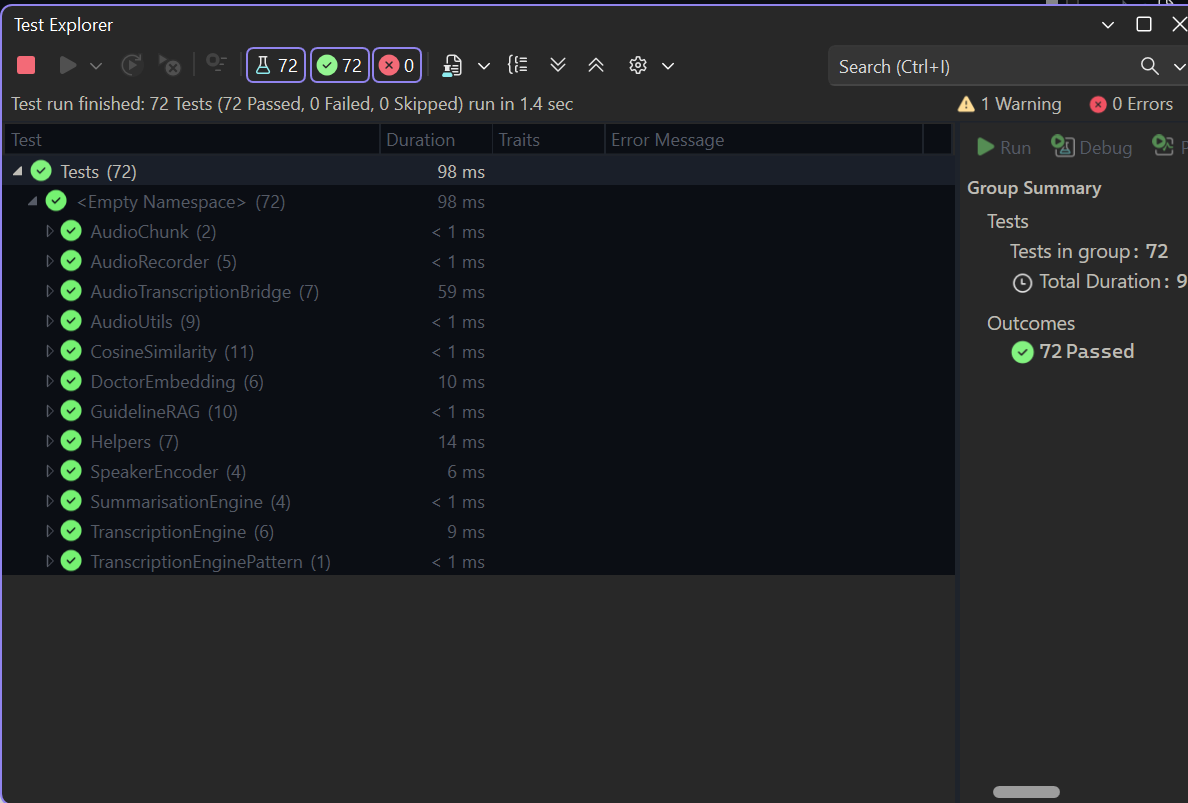
\includegraphics[width=0.5\linewidth]{unittest.png}
    \caption{All 72 unit tests passing in the Visual Studio Test Viewer}
    \label{fig:unittest_results}
\end{figure}

\section{Unit Test Cases}
\begingroup
\footnotesize % Reduces the font size for everything inside this group
\begin{longtable}{|p{0.32\textwidth}|p{0.53\textwidth}|c|}
\hline
\textbf{Test Name} & \textbf{Description} & \textbf{Pass} \\
\hline
\endfirsthead

\hline
\textbf{Test Name} & \textbf{Description} & \textbf{Pass} \\
\hline
\endhead

% --- AudioRecorder ---
\hline
\multicolumn{3}{|c|}{\textbf{AudioRecorder}} \\
\hline
DelegatesStartToBackend & Verifies audio recorder delegates Start to injected backend. & Yes \\ \hline
DelegatesStopToBackend & Verifies audio recorder delegates Stop to injected backend. & Yes \\ \hline
DelegatesStartMultipleTimes & Verifies backend start can be called multiple times. & Yes \\ \hline
DelegatesStopWithoutStart & Verifies backend stop can be called safely without a prior start. & Yes \\ \hline
DelegatesStartThenStop & Verifies start and stop both route through seam on same instance. & Yes \\ \hline

% --- AudioTranscriptionBridge ---
\hline
\multicolumn{3}{|c|}{\textbf{AudioTranscriptionBridge}} \\
\hline
PushAndPopSingleChunk & Verifies single chunk roundtrip. & Yes \\ \hline
FIFOOrdering & Verifies FIFO ordering. & Yes \\ \hline
PopBlocksUntilPush & Verifies blocking pop. & Yes \\ \hline
EmptyAudioDataChunk & Verifies empty payload handling. & Yes \\ \hline
PreservesIsLastFalse & Verifies false isLast flag is preserved through queueing. & Yes \\ \hline
PreservesOrderAndLastMarker & Verifies two-chunk order and final marker are preserved. & Yes \\ \hline
PopsPreBufferedItems & Verifies pop can consume pre-buffered multiple items without blocking. & Yes \\ \hline
ConcurrentProducersComplete & Verifies concurrent producers preserve total item count. & Yes \\ \hline

% --- AudioUtils ---
\hline
\multicolumn{3}{|c|}{\textbf{AudioUtils}} \\
\hline
NormaliseScalesMidAmplitude & Verifies scaling path. & Yes \\ \hline
NormaliseSkipsQuietAudio & Verifies quiet threshold path. & Yes \\ \hline
NormaliseSkipsAlreadyLoudAudio & Verifies loud threshold path. & Yes \\ \hline
NormaliseSkipsLowerBoundary & Verifies lower boundary max\_amp==0.001 is not scaled. & Yes \\ \hline
NormaliseSkipsUpperBoundary & Verifies upper boundary max\_amp==0.9 is not scaled. & Yes \\ \hline
NormalisePreservesSigns & Verifies normalization keeps sample signs intact. & Yes \\ \hline
NormaliseHandlesEmptyBuffer & Verifies empty audio buffers are handled safely. & Yes \\ \hline
NormaliseSingleSample & Verifies single sample normalization reaches target amplitude. & Yes \\ \hline
NormaliseAllZerosNoChange & Verifies normalization keeps zeros unchanged. & Yes \\ \hline

% --- CosineSimilarity ---
\hline
\multicolumn{3}{|c|}{\textbf{CosineSimilarity}} \\
\hline
IdenticalVectors & Verifies cosine=1 for identical vectors. & Yes \\ \hline
OrthogonalVectors & Verifies orthogonal vectors. & Yes \\ \hline
OppositeVectors & Verifies opposite vectors. & Yes \\ \hline
DifferentSizesReturnZero & Verifies mismatch branch. & Yes \\ \hline
EmptyVectorsReturnZero & Verifies empty branch. & Yes \\ \hline
ZeroVectorReturnZero & Verifies zero denominator branch. & Yes \\ \hline
ScaledDirection & Verifies scale invariance. & Yes \\ \hline
SymmetricResult & Verifies cosine similarity is symmetric. & Yes \\ \hline
OneDimensionalPositive & Verifies one-dimensional positive vectors return full similarity. & Yes \\ \hline
OneDimensionalOpposite & Verifies one-dimensional opposite vectors return negative similarity. & Yes \\ \hline
MixedSignsWithinBounds & Verifies mixed sign vectors produce bounded similarity. & Yes \\ \hline

% --- DoctorEmbedding ---
\hline
\multicolumn{3}{|c|}{\textbf{DoctorEmbedding}} \\
\hline
SetStorageDirectoryAndProfileFlagPath & Verifies doctor embedding stores override directory. & Yes \\ \hline
DelegatesEnrollAndSaveToBackend & Verifies doctor embedding delegates enrollment capture and save to injected backend. & Yes \\ \hline
DelegatesLoadToBackend & Verifies doctor embedding delegates load path through backend when memory cache is empty. & Yes \\ \hline
EmptyCapturedAudioSkipsSave & Verifies enrollment with empty captured audio does not save profile. & Yes \\ \hline
LoadFromBackendIsCached & Verifies loading from backend is cached after first fetch. & Yes \\ \hline
UsesBackendDefaultPathForSave & Verifies backend default path is used when no storage override is set. & Yes \\ \hline

% --- GuidelineRAG ---
\hline
\multicolumn{3}{|c|}{\textbf{GuidelineRAG}} \\
\hline
UsesInjectedBackendForInitialize & Verifies initialize delegation through interface seam. & Yes \\ \hline
UsesInjectedBackendForEmbedText & Verifies embed delegation through seam. & Yes \\ \hline
UsesInjectedBackendForQuery & Verifies query delegation through seam. & Yes \\ \hline
UsesInjectedBackendForReload & Verifies reload delegation through seam. & Yes \\ \hline
UsesInjectedBackendForHasIndex & Verifies has-index delegation through seam. & Yes \\ \hline
QueryReturnsEmptyWhenNoBackend... & Verifies null-impl safe path. & Yes \\ \hline
QueryForwardsInputAndTopK & Verifies query text and topK are forwarded to injected backend. & Yes \\ \hline
EmbedTextForwardsInput & Verifies embed text is forwarded to injected backend. & Yes \\ \hline
QueryUsesDefaultTopKWhenOmitted & Verifies default topK value is forwarded when omitted. & Yes \\ \hline
HasIndexFalseFromBackend & Verifies backend false index state is reflected by wrapper. & Yes \\ \hline
HasIndexReflectsBackendToggle & Verifies backend true index state can be toggled after injection. & Yes \\ \hline

% --- Helpers ---
\hline
\multicolumn{3}{|c|}{\textbf{Helpers}} \\
\hline
GetModelPathWithOverride & Verifies override path usage. & Yes \\ \hline
GetModelPathSubfolder & Verifies slash normalization. & Yes \\ \hline
GetGuidelinesDataPathCreatesFolder & Verifies directory creation branch. & Yes \\ \hline
OverrideCanBeCleared & Verifies clear override behavior. & Yes \\ \hline
GetGuidelinesDataPathStable... & Verifies same override returns same data folder path each call. & Yes \\ \hline
GetModelPathNestedSegments & Verifies nested model path joining works. & Yes \\ \hline
GetGuidelinesDataPathSuffix & Verifies guidelines data path points to guidelines\_data suffix. & Yes \\ \hline

% --- AudioChunk ---
\hline
\multicolumn{3}{|c|}{\textbf{AudioChunk}} \\
\hline
DefaultIsNotLast & Verifies default isLastChunk value. & Yes \\ \hline
DefaultAudioIsEmpty & Verifies default audio vector empty. & Yes \\ \hline
AudioDataCanBeAssigned & Verifies chunk audio is mutable as expected. & Yes \\ \hline

% --- SpeakerEncoder ---
\hline
\multicolumn{3}{|c|}{\textbf{SpeakerEncoder}} \\
\hline
DelegatesInitializeToBackend & Verifies speaker encoder delegates initialization to injected backend. & Yes \\ \hline
DelegatesEmbeddingToBackend & Verifies speaker encoder delegates embedding to injected backend. & Yes \\ \hline
DelegatesEmptyEmbedding & Verifies encoder can return empty embeddings from backend. & Yes \\ \hline
RepeatedInitializeUpdatesArgs & Verifies repeated initialize calls update backend args. & Yes \\ \hline
EmbeddingCapturesSingleSampleInput & Verifies embedding input is captured exactly for boundary-size vectors. & Yes \\ \hline

% --- SummarisationEngine ---
\hline
\multicolumn{3}{|c|}{\textbf{SummarisationEngine}} \\
\hline
DelegatesLoadModelToBackend & Verifies summarisation load delegates model path to injected backend. & Yes \\ \hline
DelegatesGenerateToBackend & Verifies summarisation prompt and generation parameters are forwarded to backend. & Yes \\ \hline
HandlesEmptyBackendOutput & Verifies summarisation backend can return empty output. & Yes \\ \hline
ForwardsMultilineTranscript & Verifies multiline transcript is forwarded into prompt. & Yes \\ \hline
IncludesSystemPromptHeader & Verifies system prompt header is included. & Yes \\ \hline
IncludesAssistantMarker & Verifies assistant marker is included in composed prompt. & Yes \\ \hline
HandlesEmptyTranscriptInput & Verifies empty transcript still composes a valid prompt. & Yes \\ \hline

% --- TranscriptionEngine ---
\hline
\multicolumn{3}{|c|}{\textbf{TranscriptionEngine}} \\
\hline
CancelDuringLoopReturnsEmpty & Verifies cancellation while loop is waiting returns empty transcript. & Yes \\ \hline
LabelsDoctorWithHighSimilarity & Verifies transcription engine labels a long segment as doctor when similarity is high. & Yes \\ \hline
LabelsPatientWithLowSimilarity & Verifies transcription engine labels a long segment as patient when similarity is low. & Yes \\ \hline
KeepsUnknownForShortSegments & Verifies transcription engine keeps unknown label for short segments. & Yes \\ \hline
InitialiseModelDelegatesPath & Verifies transcription backend model initialization path is passed through. & Yes \\ \hline
AppendsMultipleChunks & Verifies multiple generated chunks are appended into transcript. & Yes \\ \hline
IsCancelledReflectsState & Verifies cancellation flag accessor reflects cancellation calls. & Yes \\ \hline
GenerateCalledForInputChunk & Verifies generated chunks function is invoked once per input chunk. & Yes \\ \hline
OutOfRangeTimestampsAreClamped & Verifies out-of-range timestamps do not crash and still produce output line. & Yes \\ \hline
\end{longtable}
\endgroup
\chapter{User Interface Testing}
\ref{app:ui_test}

TODO
\chapter{Medical Transcription Results}
\label{app:testing_transcription_results}

\begin{table}[H] % 'H' forces the table to stay exactly here
\centering
\footnotesize % Reduced font size to fit more vertically
\renewcommand{\arraystretch}{0.8} % Compresses vertical space between rows

% --- FIRST COLUMN ---
\begin{minipage}[t]{0.48\textwidth}
\centering
\begin{tabular}{|l|l|c|}
\hline
\textbf{Real Word} & \textbf{Transcription} & \textbf{Correct} \\ \hline
Abdomen & Abdomen & Y \\ \hline
Ablation & Ablation & Y \\ \hline
Absence seizure & Absence seizure & Y \\ \hline
Acute & Acute & Y \\ \hline
Bacteraemia & Bacteremia & N (Inacc.) \\ \hline
Bacteriostatic & Bacteriostatic & Y \\ \hline
Bell's palsy & Bells palsy & N (Inacc.) \\ \hline
Bilirubin & Bilirubin & Y \\ \hline
Cachexia & Cachexia & Y \\ \hline
Calcitonin & Calcitonin & Y \\ \hline
Cannula & Cannula & Y \\ \hline
Capsid & Capsid & Y \\ \hline
Dander & Dander & Y \\ \hline
Delirium & Delirium & Y \\ \hline
Dementia & Dementia & Y \\ \hline
Dermatitis & Dermatitis & Y \\ \hline
Eczema & Eczema & Y \\ \hline
Efficacy & Efficacy & Y \\ \hline
Embolism & Embolism & Y \\ \hline
Encephalitis & Encephalitis & Y \\ \hline
Fatigue & Fatigue & Y \\ \hline
Febrile & Febrile & Y \\ \hline
Fibrillation & Fibrillation & Y \\ \hline
Fissure & Fisher & N (Incor.) \\ \hline
Gangrene & Gangrene & Y \\ \hline
Gastritis & Gastritis & Y \\ \hline
Glaucoma & Glaucoma & Y \\ \hline
Glucose & Glucose & Y \\ \hline
Haematoma & Hematoma & N (Inacc.) \\ \hline
Haemoglobin & Hemoglobin & N (Inacc.) \\ \hline
Haemophilia & Hemophilia & N (Inacc.) \\ \hline
Hay fever & Hay fever & Y \\ \hline
Idiopathic & Idiopathic & Y \\ \hline
Ileus & Ileus & Y \\ \hline
Immunity & Immunity & Y \\ \hline
Insomnia & Insomnia & Y \\ \hline
Jaundice & Jaundice & Y \\ \hline
Joint pain & Joint pain & Y \\ \hline
Jugular vein & Jugular vein & Y \\ \hline
Juvenile & Juvenile & Y \\ \hline
Keratitis & Keratitis & Y \\ \hline
Ketoacidosis & Ketoacidosis & Y \\ \hline
Kidney stone & Kidney stone & Y \\ \hline
Kinase & Kinase & Y \\ \hline
Larynx & Larynx & Y \\ \hline
Laxatives & Laxatives & Y \\ \hline
Lesion & Lesion & Y \\ \hline
Leukaemia & Leukemia & N (Inacc.) \\ \hline
Macula & Macula & Y \\ \hline
Malaise & Malaise & Y \\ \hline
Malignant & Malignant & Y \\ \hline
Metastasis & Metastasis & Y \\ \hline
\end{tabular}
\end{minipage}\hfill
% --- SECOND COLUMN ---
\begin{minipage}[t]{0.48\textwidth}
\centering
\begin{tabular}{|l|l|c|}
\hline
\textbf{Real Word} & \textbf{Transcription} & \textbf{Correct} \\ \hline
Narcolepsy & Narcolepsy & Y \\ \hline
Nausea & Nausea & Y \\ \hline
Necrosis & Necrosis & Y \\ \hline
Neonate & Neonate & Y \\ \hline
Obesity & Obesity & Y \\ \hline
Ocular & Ocular & Y \\ \hline
Oedema & Oedema & Y \\ \hline
Oestrogen & Estrogen & N (Inacc.) \\ \hline
Palpitations & Palpitations & Y \\ \hline
Pancreatitis & Pancreatitis & Y \\ \hline
Paraesthesia & Paresthesia & N (Inacc.) \\ \hline
Pruritus & Pruritus & Y \\ \hline
QT interval & QT interval & Y \\ \hline
Quadriplegia & Quadriplegia & Y \\ \hline
Queasiness & Queasiness & Y \\ \hline
Quinsy & Quinsy & Y \\ \hline
Radiotherapy & Radiotherapy & Y \\ \hline
Receptor & Receptor & Y \\ \hline
Relapse & Relapse & Y \\ \hline
Remission & Remission & Y \\ \hline
Sedation & Sedation & Y \\ \hline
Seizure & Seizure & Y \\ \hline
Shingles & Shingles & Y \\ \hline
Syncope & Sync up & N (Incor.) \\ \hline
Tachycardia & Tachycardia & Y \\ \hline
Tinnitus & Tinnitus & Y \\ \hline
Tonsillitis & Tonsillitis & Y \\ \hline
Tophi & Trophy & N (Incor.) \\ \hline
Ulcer & Ulcer & Y \\ \hline
Urethra & Urethra & Y \\ \hline
Urticaria & Urticaria & Y \\ \hline
Uterus & Uterus & Y \\ \hline
Vaccine & Vaccine & Y \\ \hline
Varicella & Varicella & Y \\ \hline
Vascular & Vascular & Y \\ \hline
Vertigo & Vertigo & Y \\ \hline
Warts & Warts & Y \\ \hline
Wasting & Wasting & Y \\ \hline
Weakness & Weakness & Y \\ \hline
Wheezing & Wheezing & Y \\ \hline
X-ray & X-ray & Y \\ \hline
Xanthoma & Xanthoma & Y \\ \hline
Xenograft & Xenograft & Y \\ \hline
Xerosis & Xerosis & Y \\ \hline
Yawning & Yawning & Y \\ \hline
Yeast infection & Yeast infection & Y \\ \hline
Yellow fever & Yellow fever & Y \\ \hline
Yersiniosis & Yersiniosis & Y \\ \hline
Zoonosis & Zoonosis & Y \\ \hline
Zoster & Zoster & Y \\ \hline
Zygote & Zygote & Y \\ \hline
Zymotic & Zymotic & Y \\ \hline
\end{tabular}
\end{minipage}

\caption{Detailed Transcription Accuracy Results (A-Z)}
\label{tab:test_transcription}
\end{table}
\chapter{User Manual}
\label{app:user_manual}
The workflow for this application is generally linear. Upon loading the application, the user will be greeted by an "Enroll Doctor's Voice" screen, which is used to calculate and store the voice signature of the doctor to compare against a patient's voice providing accurate speaker labels for the transcription. This is a one time event; unless the user wishes to re-record the voice signature or hand the device to another doctor this process will not be required again. Once completed, the user is greeted with the "Ready to record" screen. By pressing "Start Recording", the conversation will be recorded. When pressing "Stop Recording" the application will summarise the conversation. This summary can be copied to the clipboard and saved to an external file. An appraisal entry can be generated by pressing "Create Appraisal Entry" and completing and saving the dialogue and optionally saved to an external text file. By pressing the "Appraisal History" button, the appraisals history page allows appraisals to be viewed, edited and deleted, searched and filtered. In the settings, medical guidance PDF documents can be uploaded from the user's computer to enable guideline retrieval. On the summarisation screen, pressing "View Guidance" will search the guidance for the most relevant guidelines based on the summarisations. These can be viewed within the PDF viewing window. Finally, the settings menu enables microphone switching, re-enrollment of the doctors voice, changing of the default save location and deleting all appraisals. Finally, the help button provides more guidance on how to use the application and the information button provides the legal disclaimer.
\chapter{System Manual}
\label{app:system_manual}
\section{Environment}
To download the application for development, use the google drive link and unzip the folder. This application must be developed on Microsoft Visual Studio 2026 edition due to the MSIX sandbox environment. The root folder contains 4 main folders. The External folder holds all library \texttt{.lib}, \texttt{.bin} and \texttt{.dll} files. The ClinicalSummarisation folder holds all written code and Clinical Summarisation (Package) holds all packaged models. Finally, the Tests folder holds all unit test code. 

To open the development environment, double click the \texttt{ClinicalSummarisation.slnx} file. To run the program, right click on the top file in the solution explorer and select deploy. To run the tests for the program, click on the view button at the very top of the page and select Test Viewer. Press the green play symbol to run the tests. 
\chapter{Other appendices, e.g., code listing}
Put your appendix sections here
\end{document}